\documentclass[a4paper,11pt]{article}
\usepackage[utf8]{inputenc}
\usepackage[T1]{fontenc}
\usepackage{geometry}\geometry{margin=2.2cm}
\usepackage{amsmath,amssymb,amsthm}
\usepackage{tikz}
\usetikzlibrary{arrows.meta,positioning,shapes,calc,backgrounds,
  decorations.pathreplacing,matrix,fit,patterns}
\usepackage{pgfplots}
\pgfplotsset{compat=1.18}
\usepackage{booktabs,array,colortbl,xcolor,mdframed,enumitem,caption,float}
\usepackage{eurosym}
\usepackage[hyphens]{url}
\usepackage[round,authoryear,sort&compress]{natbib}
\usepackage[colorlinks=true,linkcolor=matblue,citecolor=tealcol,urlcolor=matblue]{hyperref}
\usepackage{algorithm}
\usepackage{algpseudocode}
\usepackage{appendix}

% ── Farben ──────────────────────────────────────────────────
\definecolor{matblue}{RGB}{83,74,183}
\definecolor{matlight}{RGB}{238,237,254}
\definecolor{tealcol}{RGB}{15,110,86}
\definecolor{teallight}{RGB}{225,245,238}
\definecolor{ambercol}{RGB}{186,117,23}
\definecolor{amberlight}{RGB}{250,238,218}
\definecolor{redcol}{RGB}{162,45,45}
\definecolor{redlight}{RGB}{252,235,235}
\definecolor{graycol}{RGB}{95,94,90}
\definecolor{graylight}{RGB}{241,239,232}
\definecolor{greencol}{RGB}{39,80,10}
\definecolor{greenlight}{RGB}{234,243,222}

% Heatmap-Farben (7 Stufen)
\definecolor{heat0}{RGB}{255,255,255}   % 0
\definecolor{heat1}{RGB}{230,245,255}   % 0–0.5
\definecolor{heat2}{RGB}{180,220,250}   % 0.5–1.0
\definecolor{heat3}{RGB}{120,185,230}   % 1.0–1.5
\definecolor{heat4}{RGB}{70,140,200}    % 1.5–2.0
\definecolor{heat5}{RGB}{30,90,160}     % >2.0
\definecolor{heat5txt}{RGB}{255,255,255}

\newtheorem{definition}{Definition}
\newtheorem{satz}{Satz}
\newtheorem{lemma}{Lemma}

\floatname{algorithm}{Algorithmus}
\renewcommand{\algorithmicrequire}{\textbf{Eingabe:}}
\renewcommand{\algorithmicensure}{\textbf{Ausgabe:}}

% ────────────────────────────────────────────────────────────
\title{\textbf{Verdrängungsimpuls und Ersetzungswert:\\
Eine relationale Matrixmethode\\
für das 0/1-Knapsack-Problem}\\[0.3em]
\large Formale Herleitung, konstruiertes Gegenbeispiel,\\
Frequenzanalyse und Vergleich mit 8~Methoden}
\author{Dogan Balban\\[0.3em]
\small Independent Researcher\\
\small \texttt{}}
\date{März 2026}

\begin{document}
\maketitle

% ── Abstract ────────────────────────────────────────────────
\begin{abstract}
\noindent
Wir führen den \emph{Matrix-Score} ein, eine neuartige relationale
Heuristik für das 0/1-Knapsack-Problem, die auf einer
$n\times n$-Proportionsmatrix basiert. In dieser Matrix wird jede
Ware gleichzeitig als Container und als Inhalt betrachtet: die
Zelle $M[i][j]$ misst, wie viele Exemplare von Ware~$j$
gewichtsmäßig in den Container~$i$ passen und welchen relativen
Wert diese Befüllung ergibt.
Obwohl die zentrale Matrixzelle auf dem
UKP-Operator $\lfloor w_i/w_j \rfloor$ basiert -- der
Simple-Dominance-Zahl aus der Unbounded-Knapsack-Literatur --
verwenden wir ihn nicht zur Eliminierung dominierter Items,
sondern als Baustein einer relationalen Bewertung im 0/1-Kontext.
Während klassische Greedy-Verfahren eine eindimensionale Größe
(Effizienz $v/w$) optimieren, sucht der Matrix-Score den
Gleichgewichtspunkt zwischen dem Nutzwert einer Ware und ihrem
strukturellen Verdrängungsimpuls innerhalb des Warenkollektivs.
Der daraus abgeleitete Kern-Score $\bar{M}_j$ -- der mittlere
Ersetzungswert über alle aufnehmenden Container -- ist
parameterfrei, hat Komplexität $\mathcal{O}(n^2)$ und ist
\emph{unabhängig} von der Rucksackkapazität~$W$.

Wir stellen die vollständige formale Herleitung vor, zeigen die
Berechnung an einem durchgerechneten 7-Waren-Beispiel mit
farbkodierter Heatmap, geben einen konstruierten Gegenfall an,
in dem der reine Kern-Score $\bar{M}_j$ -- ohne empirische
Parameter -- das DP-Optimum findet, wo die $v/w$-Heuristik
versagt, analysieren die Frequenzsignatur der Auswahlmethoden
mittels Diskreter Fourier-Transformation und untersuchen die
Laufzeitcharakteristik der reinen relationalen Berechnung
im Vergleich zu wertbasierten Varianten.
\end{abstract}

\tableofcontents
\bigskip

% ═══════════════════════════════════════════════════════════
\section{Einleitung und Motivation}

Das 0/1-Knapsack-Problem gehört zu den meistuntersuchten NP-schweren
Optimierungsproblemen der Kombinatorik -- erste formale Arbeiten reichen
bis in das Jahr 1897 zurück \citep{kellerer2004}.
Gegeben $n$ Waren mit Wert $v_i$ und Gewicht $w_i$ sowie eine
Kapazität $W$, wähle $S \subseteq \{1,\ldots,n\}$,
sodass $\sum_{i\in S} w_i \le W$ und $\sum_{i\in S} v_i$ maximiert wird.

\medskip
Zwei Paradigmen dominieren die Literatur:
\begin{itemize}[leftmargin=*,topsep=2pt]
  \item \textbf{Greedy-Heuristiken} -- sortieren Waren nach einem Kriterium
    und wählen gierig. Der Greedy-Algorithmus nach Wert-Gewicht-Verhältnis
    $v_i/w_i$ wurde von \citet{dantzig1957} eingeführt; neuere Varianten
    wurden von \citet{hristakeva2005,hristakeva2023} verglichen.
  \item \textbf{Exakte Verfahren} -- Dynamic Programming in
    $\mathcal{O}(n\cdot W)$ \citep{bellman1957}, Branch \& Bound
    \citep{kolesar1967}, sowie das FPTAS von \citet{ibarra1975}.
    Die umfassendste Referenz bleibt \citet{kellerer2004};
    neuere Übersichten liefern \citet{cacchiani2022}.
\end{itemize}

\noindent
Allen Greedy-Methoden ist gemeinsam, dass sie jede Ware
\emph{isoliert} bewerten -- nach $v_i$, nach $w_i$ oder nach $v_i/w_i$.
Keiner dieser Scores berücksichtigt, wie Waren \emph{zueinander stehen}:
ob eine schwere Ware den Platz zweier leichterer blockiert,
oder ob viele kleine Waren eine große ersetzen können.

\medskip
\noindent
\textbf{Kernfrage dieser Arbeit.}
Kann man aus den \emph{paarweisen Proportionsverhältnissen}
aller Waren einen Score ableiten, der diese strukturelle Information
nutzt -- ohne die Kapazität $W$ zu kennen?

\medskip
\noindent
\textbf{Beitrag.}
Wir führen den \emph{Matrix-Score} ein: eine $n\times n$-Proportionsmatrix,
in der jede Ware gleichzeitig als Container und als Inhalt betrachtet wird.
Die zentrale Matrixzelle nutzt den UKP-Operator
$\lfloor w_i/w_j \rfloor$ -- bekannt als Simple-Dominance-Zahl
\citep{kellerer2004} -- nicht zur Eliminierung dominierter Items,
sondern als Baustein einer relationalen Bewertung im 0/1-Kontext.
Diese Perspektive ist in der Literatur nicht vorhanden und kombiniert
drei Eigenschaften:

\begin{enumerate}[leftmargin=*,topsep=2pt]
  \item $W$-Unabhängigkeit des Scores,
  \item relationale (paarweise) Bewertung aller Waren,
  \item Einsatzfähigkeit als relationale Heuristik und Analysewerkzeug.
\end{enumerate}

% ═══════════════════════════════════════════════════════════
\section{Verwandte Arbeiten}

\subsection{Greedy-Varianten}

\citet{dantzig1957} bewies Optimalität für das \emph{fraktionale}
Knapsack-Problem. Für das 0/1-Problem kann die Approximationsgarantie
beliebig schlecht werden \citep{kellerer2004}.
\citet{hristakeva2005} vergleichen systematisch drei Greedy-Strategien
(Sortierung nach Wert, nach Gewicht, nach $v/w$) und zeigen, dass
$v/w$ die beste mittlere Performance liefert.
\citet{hristakeva2023} führen \emph{Max-of-Two} und
\emph{Defensive Greedy} ein und verbessern die Approximationsgüte
auf ca.\ 99\,\% des Optimums, bei unveränderter
$\mathcal{O}(n\log n)$-Komplexität.

\subsection{Exakte und approximative Verfahren}

Das expandierende Core-Konzept von \citet{pisinger1995,pisinger1997}
reduziert den DP-Suchraum auf eine minimale Teilmenge.
\citet{pisinger2005} klassifiziert Instanzen in unkorrellierte,
schwach und stark korrellierte Klassen -- eine Taxonomie, die wir
für unsere empirische Analyse übernehmen.
\citet{plateau1982} entwickelten den ersten hybriden B\&B+DP-Ansatz;
\citet{balev2008} erweitern dies auf mehrdimensionale Probleme.

\subsection{Dominanz und Paarvergleiche}

\citet{andonov2000} zeigen: Threshold-Dominanz der Form
$\lfloor w_i/w_j \rfloor$ kann als Preprocessing den UKP-Suchraum
um Größenordnungen verkleinern. \citet{smithmiles2021} nutzen
$\mathcal{O}(n^2)$ paarweise Vergleiche als
Instanzcharakterisierungs-Features.
Unser Matrix-Score ist strukturell verwandt, verfolgt aber das
Ziel der \emph{Lösungsfindung} statt der Instanzklassifikation.

\subsection{UKP-Operator im 0/1-Kontext}
\label{sec:ukp}

Obwohl wir das \emph{0/1}-Knapsack-Problem betrachten, basiert
die Matrixzelle
\[
M[i][j] = \lfloor w_i/w_j \rfloor \cdot v_j/v_i
\]
strukturell auf einem \emph{UKP-Operator}: der ganzzahligen
Kapazitätszahl $\lfloor w_i/w_j \rfloor$ erlaubt konzeptionell
mehrere Kopien von Ware~$j$ im Container~$i$ -- eine Operation,
die im 0/1-Problem nicht zulässig ist, im Unbounded Knapsack
Problem (UKP) aber die zentrale Größe darstellt.

\medskip
\noindent
In der UKP-Literatur wird $\lfloor w_i/w_j \rfloor$ als
\emph{Simple-Dominance-Zahl} \citep{kellerer2004} bzw.\
\emph{Threshold-Dominanz-Zahl} \citep{andonov2000} zur
\textbf{Eliminierung} dominierter Items verwendet.
Wir verwenden diesen Operator jedoch nicht zur Elimination,
sondern als \textbf{Baustein einer relationalen Bewertung}:
die Zahl $\lfloor w_i/w_j \rfloor$ quantifiziert, wie viel
strukturelle Evidenz Container~$i$ für die Nützlichkeit von
Ware~$j$ liefert.

\medskip
\noindent
Dadurch entsteht ein \emph{UKP-informierter Informationsfluss
innerhalb eines 0/1-Problems}: leichte Waren, die in viele
Container passen ($|\mathcal{C}_j|$ groß, hohe
$\lfloor w_i/w_j \rfloor$-Werte), akkumulieren mehr relationale
Evidenz als schwere Waren mit wenigen Containern.
Diese Perspektive erklärt drei zentrale Eigenschaften des
Matrix-Scores:
\begin{itemize}[topsep=2pt]
  \item \textbf{$W$-Unabhängigkeit}: der UKP-Operator
    $\lfloor w_i/w_j \rfloor$ ist rein item-relational und
    benötigt keine Kapazitätsangabe.
  \item \textbf{Blockierungserkennung}: eine schwere Ware mit
    $|\mathcal{C}_j| = 1$ (nur eigener Container) erhält
    minimal UKP-Evidenz -- ihr Score konvergiert zum
    Diagonalwert~$1$.
  \item \textbf{Strukturelle Tiefe}: der Score enthält mehr
    Information als der eindimensionale Quotient $v/w$, weil
    er die paarweise UKP-Dominanzstruktur aller Items aggregiert.
\end{itemize}

\subsection{Quadratic Knapsack Problem}

\citet{gallo1980} maximieren eine quadratische Zielfunktion mit
paarweisen Nutzentermen $p_{ij}$ -- konzeptuell dem Matrix-Score ähnlich,
aber symmetrisch und nicht auf Kapazitätsverhältnisse bezogen.

% ═══════════════════════════════════════════════════════════
\section{Formale Definition: Relationale Proportionsmatrix}
\label{sec:formal}

\subsection{Intuition}

Die zentrale Idee ist, jede Ware aus zwei Perspektiven zu betrachten:

\begin{itemize}[leftmargin=*,topsep=2pt]
  \item \textbf{Als Container:} Wie viele \emph{andere} Waren passen
    gewichtsmäßig in den Platz, den diese Ware belegt?
  \item \textbf{Als Inhalt:} Wie gut passt diese Ware in die
    ``Container'' der anderen Waren, und welchen Wert bringt sie dort?
\end{itemize}

\noindent
Eine Ware, die in viele Container passt und dabei hohen relativen
Wert liefert, ist \emph{vielseitig nützlich}. Eine Ware, deren
Container kaum andere Waren aufnehmen kann, ist potenziell
\emph{blockierend}.

\subsection{Matrixzelle}

\begin{mdframed}[backgroundcolor=matlight,linecolor=matblue,linewidth=1.2pt]
\begin{definition}[Matrixzelle]
\label{def:zelle}
Seien $n$ Waren mit Wert $v_i > 0$ und Gewicht $w_i > 0$ gegeben.
Die \emph{relationale Proportionsmatrix} $M \in \mathbb{R}^{n \times n}$
ist definiert durch:
\[
M[i][j] \;=\; \left\lfloor \frac{w_i}{w_j} \right\rfloor
\cdot \frac{v_j}{v_i},
\qquad i,j \in \{1,\ldots,n\}
\]
\end{definition}
\end{mdframed}

\medskip
\noindent
\textbf{Interpretation der Faktoren:}

\begin{itemize}[leftmargin=*,topsep=4pt]
  \item $\lfloor w_i / w_j \rfloor$ -- die
    \emph{ganzzahlige Kapazitätszahl}: wie viele Exemplare
    von Ware~$j$ gewichtsmäßig in den ``Container'' der
    Ware~$i$ passen. Dies ist exakt die Simple-Dominance-Zahl
    aus \citet{kellerer2004}, Kap.~2, und die
    Threshold-Dominanz-Zahl aus \citet{andonov2000}.
  \item $v_j / v_i$ -- das \emph{relative Wertverhältnis}: der
    Wert einer einzelnen Ware~$j$ im Verhältnis zum Wert der
    Container-Ware~$i$.
  \item $M[i][j]$ insgesamt -- der \emph{Ersetzungswert}: das
    Vielfache des Werts von Ware~$i$, das man durch Befüllung
    ihres Gewichtsplatzes mit Ware~$j$ erzielen könnte.
\end{itemize}

\medskip
\noindent
\textbf{Spezialfälle:}
\begin{itemize}[leftmargin=*,topsep=2pt]
  \item $M[i][j] = 0$, falls $w_j > w_i$ (Ware~$j$ passt nicht
    in Container~$i$).
  \item $M[i][i] = 1$ für alle $i$ (Diagonale: jede Ware passt
    genau einmal in ihren eigenen Container).
  \item $M[i][j] > 1$ bedeutet: die Befüllung mit Ware~$j$ ist
    \emph{wertvoller} als Ware~$i$ selbst.
\end{itemize}

\subsection{Matrix-Score}

\begin{mdframed}[backgroundcolor=matlight,linecolor=matblue,linewidth=1.2pt]
\begin{definition}[Matrix-Score]
\label{def:score}
Für jede Ware $j \in \{1,\ldots,n\}$ definiere die Menge der
\emph{aufnehmenden Container}:
\[
\mathcal{C}_j = \bigl\{i \in \{1,\ldots,n\} :
  \lfloor w_i/w_j \rfloor > 0\bigr\}
\]
Der \emph{Matrix-Score} von Ware $j$ ist der mittlere
Ersetzungswert über alle aufnehmenden Container:
\[
\boxed{\;
\operatorname{Score}(j) \;=\; \bar{M}_j \;=\;
\frac{1}{|\mathcal{C}_j|}
\sum_{i \in \mathcal{C}_j} M[i][j]
\;}
\]
\end{definition}
\end{mdframed}

\medskip
\noindent
\textbf{Interpretation.}
$\bar{M}_j$ misst die \emph{durchschnittliche relative Nützlichkeit}
von Ware~$j$ als Ersatz für andere Waren. Konkret:
wenn man den Gewichtsplatz einer beliebigen anderen Ware~$i$
(für die $j$ hineinpasst) mit ganzzahlig vielen Exemplaren
von $j$ befüllt, erzielt man im Mittel das $\bar{M}_j$-fache
des Werts von Ware~$i$.

\begin{itemize}[leftmargin=*,topsep=4pt]
  \item $\bar{M}_j > 1$: Ware~$j$ ist im Mittel \emph{wertvoller}
    als die Waren, deren Platz sie einnimmt -- ein Zeichen
    hoher relationaler Qualität.
  \item $\bar{M}_j < 1$: Ware~$j$ liefert im Mittel \emph{weniger}
    Wert als die Container-Waren -- sie ist relational schwach.
  \item $\bar{M}_j = 1$: Ware~$j$ ist im Mittel gleichwertig mit
    ihren Containern (die Diagonale $M[j][j]=1$ trägt hierzu bei).
\end{itemize}

\noindent
Der Score ist \emph{rein relational}: er bewertet jede Ware
ausschließlich im Verhältnis zu den anderen Waren im System,
ohne die Kapazität $W$ oder absolute Schwellenwerte zu verwenden.
Er enthält keine empirischen Koeffizienten.

\subsection{Optionale Erweiterung: Blockierungsstrafe}
\label{sec:strafe}

In Instanzen mit starken Gewichtsunterschieden kann eine schwere
Ware ($w_j \gg \bar{w}$) den Rucksack blockieren, obwohl
leichtere Waren zusammen mehr Wert liefern würden.
Der reine Score $\bar{M}_j$ erkennt dies nicht, da er nur
Container betrachtet, in die $j$ \emph{passt}, und die
Nicht-Paarungen ignoriert.

\medskip
\noindent
\textbf{Erweiterter Score.}
Sei $\mathcal{Z}_j = \{i : \lfloor w_i/w_j \rfloor = 0\}$
die Menge der Container, in die Ware~$j$ \emph{nicht} passt.
Der erweiterte Score mit Blockierungsstrafe ist:
\[
\operatorname{Score}_\alpha(j)
= \bar{M}_j \cdot
\left(1 - \alpha\,\frac{|\mathcal{Z}_j|}{n}\right),
\qquad \alpha \in [0,1]
\]

\noindent
Für $\alpha = 0$ reduziert sich der erweiterte Score auf
den Kern-Score $\bar{M}_j$. Für $\alpha > 0$ werden Waren
bestraft, die in wenige Container passen -- ein Proxy für
Blockierungspotenzial.

\medskip
\noindent
\textbf{Wann ist die Erweiterung nötig?}
Die Blockierungsstrafe verändert die Score-Rangfolge genau dann,
wenn Waren mit hohem $\bar{M}_j$ gleichzeitig hohes
$|\mathcal{Z}_j|$ aufweisen -- also Waren, die relational
wertvoll sind, aber gewichtsmäßig in wenige andere Container passen.
Dies tritt typischerweise bei Instanzen mit einem
\emph{dominanten schweren Item} auf
(vgl.\ Gegenbeispiel, Abschnitt~\ref{sec:gegen}).

\medskip
\noindent
In der empirischen Analyse (Abschnitt~\ref{sec:alpha})
zeigen wir, dass die Auswahl in vielen Instanzklassen
unabhängig von $\alpha$ ist -- der Kern-Score $\bar{M}_j$
allein liefert bereits die entscheidende Information.

\subsection{Eigenschaften}

\begin{satz}[Komplexität]
\label{satz:kompl}
Die Berechnung aller $n$ Scores erfordert $\mathcal{O}(n^2)$
Operationen und ist unabhängig von~$W$.
\end{satz}

\begin{proof}
Die Matrix $M$ hat $n^2$ Einträge, jeder in $\mathcal{O}(1)$
berechenbar (eine Ganzzahldivision, eine Multiplikation,
eine Division). Die Mengen $\mathcal{C}_j$ und $\mathcal{Z}_j$
werden beim Matrixdurchlauf mitgezählt.
Die Aggregation pro Spalte~$j$ ist in $\mathcal{O}(n)$.
Insgesamt: $\mathcal{O}(n^2)$.
Die Kapazität $W$ geht in keine Berechnung ein.
\end{proof}

\begin{satz}[Diagonale]
\label{satz:diag}
$M[i][i] = 1$ für alle $i$, d.\,h.\ jede Ware hat den
Ersetzungswert~1 für ihren eigenen Container.
\end{satz}

\begin{proof}
$M[i][i] = \lfloor w_i/w_i \rfloor \cdot v_i/v_i = 1 \cdot 1 = 1$.
\end{proof}

\begin{satz}[Asymmetrie]
\label{satz:asym}
Die Matrix $M$ ist im Allgemeinen nicht symmetrisch:
$M[i][j] \ne M[j][i]$.
Insbesondere gilt: wenn $w_j > w_i$, dann $M[i][j] = 0$,
aber $M[j][i]$ kann beliebig groß sein.
\end{satz}

\begin{proof}
Wenn $w_j > w_i$, dann $\lfloor w_i/w_j \rfloor = 0$,
also $M[i][j] = 0$.
Umgekehrt: $M[j][i] = \lfloor w_j/w_i \rfloor \cdot v_i/v_j$.
Da $w_j > w_i$, ist $\lfloor w_j/w_i \rfloor \ge 1$.
\end{proof}

\noindent
Die Asymmetrie ist keine Schwäche, sondern das zentrale
Strukturmerkmal: sie kodiert die gerichtete Beziehung
``$j$ passt in $i$, aber $i$ passt nicht in $j$''.
Dies erzeugt die UKP-informierte Hierarchie
(vgl.\ Abschnitt~\ref{sec:ukp}).

\begin{satz}[Score-Schranken]
\label{satz:bounds}
Für jede Ware $j$ gilt:
\[
\frac{v_j}{v_{\max}} \;\le\; \bar{M}_j \;\le\;
\frac{w_{\max}}{w_j} \cdot \frac{v_j}{v_{\min}}
\]
wobei $v_{\max} = \max_i v_i$, $v_{\min} = \min_i v_i$
und $w_{\max} = \max_i w_i$.
\end{satz}

\begin{proof}
\emph{Untere Schranke:}
Jeder Container $\mathcal{C}_j$ enthält mindestens $j$ selbst
(Diagonale), also $\bar{M}_j \ge M[j][j] \cdot 1/|\mathcal{C}_j|
= 1/|\mathcal{C}_j|$. Da zudem für den größten Container
$i^* = \arg\max w_i$: $M[i^*][j] = \lfloor w_{i^*}/w_j \rfloor
\cdot v_j/v_{i^*} \ge 1 \cdot v_j/v_{\max} = v_j/v_{\max}$,
folgt $\bar{M}_j \ge v_j/v_{\max}$.

\emph{Obere Schranke:}
$M[i][j] = \lfloor w_i/w_j \rfloor \cdot v_j/v_i
\le (w_i/w_j) \cdot (v_j/v_{\min})
\le (w_{\max}/w_j) \cdot (v_j/v_{\min})$.
Da $\bar{M}_j$ ein Mittelwert über solche Terme ist,
gilt die Schranke.
\end{proof}

\begin{satz}[Dominanzprinzip]
\label{satz:dom}
Wenn $\bar{M}_j > 1$, dann ist Ware~$j$ im Mittel über alle
Container wertvoller als die Container-Waren selbst.
Wenn $\bar{M}_j = 1$ und $|\mathcal{C}_j| = 1$, dann ist Ware~$j$
die schwerste Ware im System -- ihr Score basiert
ausschließlich auf dem Diagonalwert.
\end{satz}

\begin{proof}
$\bar{M}_j > 1$ bedeutet: der Mittelwert von
$\lfloor w_i/w_j \rfloor \cdot v_j/v_i$ über alle $i \in \mathcal{C}_j$
ist größer als~1. Da $M[j][j] = 1$, müssen die Beiträge
der anderen Container im Mittel $> 1$ sein.

Für $|\mathcal{C}_j| = 1$: nur $i = j$ erfüllt
$\lfloor w_i/w_j \rfloor > 0$, d.\,h.\ keine andere Ware hat
Gewicht $\ge w_j$. Also ist $j$ die schwerste Ware, und
$\bar{M}_j = M[j][j] = 1$.
\end{proof}

\begin{satz}[UKP-Verbindung]
\label{satz:ukp}
Für die reine Kapazitätsmatrix $K[i][j] = \lfloor w_i/w_j \rfloor$
entspricht der Spaltenmittelwert
$\bar{K}_j = \frac{1}{|\mathcal{C}_j|}\sum_{i \in \mathcal{C}_j}
K[i][j]$
der mittleren UKP-Packungshäufigkeit von Ware~$j$.
Es gilt:
\[
\bar{K}_j \ge 1 \quad \text{für alle } j
\]
mit Gleichheit genau dann, wenn $j$ die schwerste Ware ist
($|\mathcal{C}_j| = 1$).
\end{satz}

\begin{proof}
Da $K[j][j] = \lfloor w_j/w_j \rfloor = 1$ und alle
$K[i][j] \ge 1$ für $i \in \mathcal{C}_j$, ist
$\bar{K}_j \ge 1$.
Gleichheit gilt genau dann, wenn $\mathcal{C}_j = \{j\}$
und $K[j][j] = 1$.
\end{proof}

\subsection{Sensitivität der Blockierungsstrafe}
\label{sec:alpha}

Wir untersuchen empirisch, ob die optionale Blockierungsstrafe
(Abschnitt~\ref{sec:strafe}) die Score-Rangfolge gegenüber
dem reinen Kern-Score $\bar{M}_j$ verändert.
Dazu parametrisieren wir $\alpha \in [0,1]$:
\[
\operatorname{Score}_\alpha(j)
= \bar{M}_j \cdot \left(1 - \alpha\,\frac{|\mathcal{Z}_j|}{n}\right)
\]

\begin{center}
\small
\renewcommand{\arraystretch}{1.15}
\begin{tabular}{cl cc ccccccc}
\toprule
& & & & \multicolumn{7}{c}{Score bei Strafkoeffizient $\alpha$} \\
\cmidrule(lr){5-11}
$j$ & Ware & $\bar{M}_j$ & $\frac{|\mathcal{Z}_j|}{n}$
  & $\mathbf{\alpha{=}0}$ & $0{,}1$ & $0{,}2$ & $0{,}4$
  & $0{,}6$ & $0{,}8$ & $1{,}0$ \\
\midrule
6 & Uhr      & 1{,}478 & 0/7 &
  \textbf{1{,}478} & 1{,}478 & 1{,}478 & 1{,}478 & 1{,}478 & 1{,}478 & 1{,}478 \\
4 & Armband  & 1{,}163 & 1/7 &
  \textbf{1{,}163} & 1{,}146 & 1{,}130 & 1{,}096 & 1{,}063 & 1{,}030 & 0{,}997 \\
3 & Schmuck  & 1{,}140 & 2/7 &
  \textbf{1{,}140} & 1{,}107 & 1{,}074 & 1{,}009 & 0{,}944 & 0{,}879 & 0{,}814 \\
7 & Skulptur & 1{,}000 & 6/7 &
  \textbf{1{,}000} & 0{,}914 & 0{,}829 & 0{,}657 & 0{,}486 & 0{,}314 & 0{,}143 \\
2 & Kamera   & 0{,}955 & 3/7 &
  \textbf{0{,}955} & 0{,}914 & 0{,}873 & 0{,}791 & 0{,}709 & 0{,}628 & 0{,}546 \\
1 & Laptop   & 0{,}917 & 5/7 &
  \textbf{0{,}917} & 0{,}851 & 0{,}786 & 0{,}655 & 0{,}524 & 0{,}393 & 0{,}262 \\
5 & Tablet   & 0{,}822 & 4/7 &
  \textbf{0{,}822} & 0{,}775 & 0{,}728 & 0{,}634 & 0{,}540 & 0{,}446 & 0{,}352 \\
\bottomrule
\end{tabular}
\end{center}

\noindent
Die Tabelle ist nach dem Kern-Score $\bar{M}_j$ sortiert
(Spalte $\alpha=0$, fett). Dies ist die \emph{natürliche}
Rangfolge der Proportionsmatrix ohne jeden Zusatzparameter.

\begin{center}
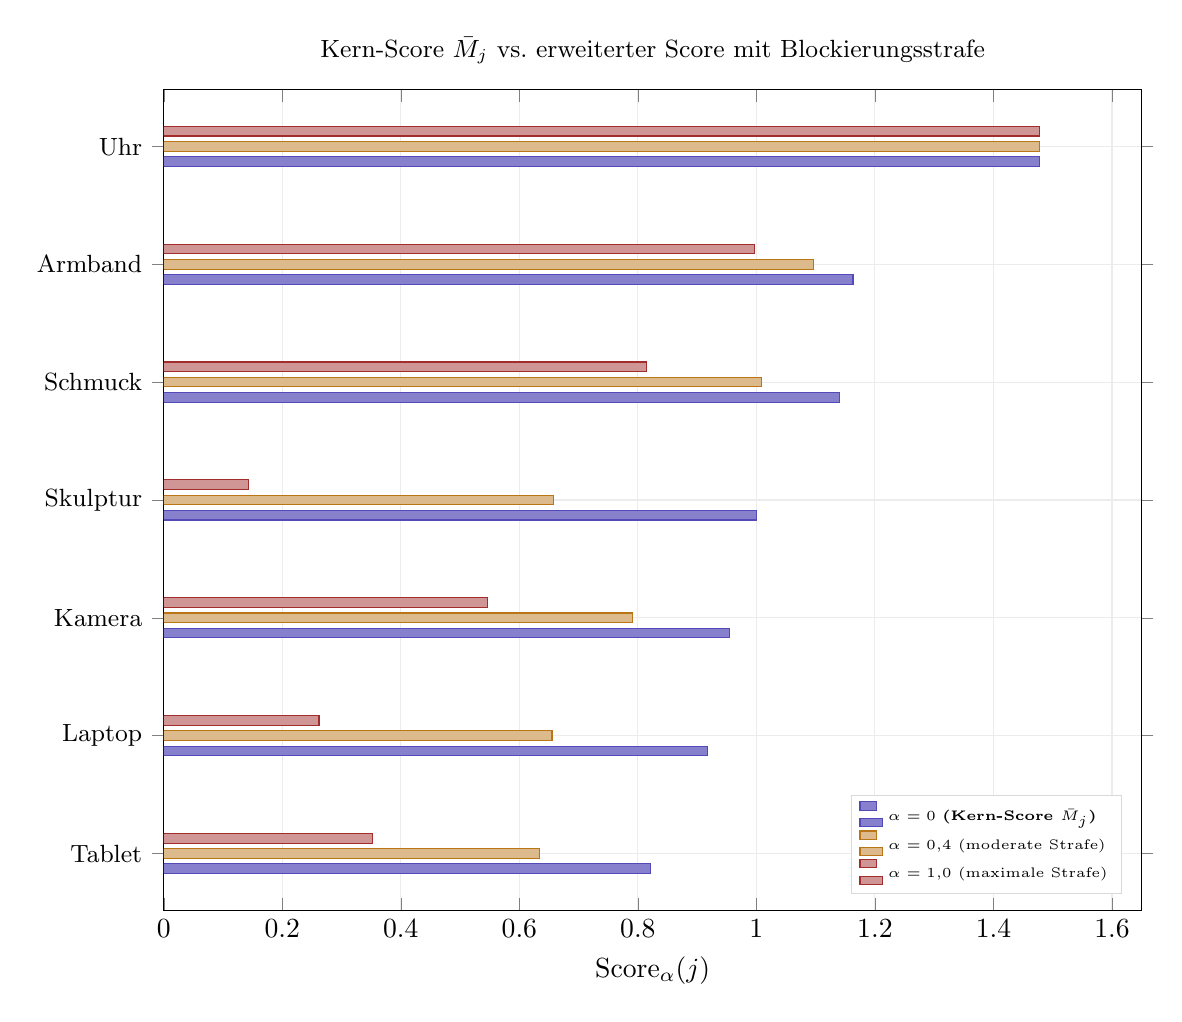
\begin{tikzpicture}
\begin{axis}[
  xbar,
  width=14cm, height=12cm,
  bar width=3.5pt,
  enlarge y limits=0.08,
  xlabel={$\operatorname{Score}_\alpha(j)$},
  symbolic y coords={
    Tablet,Laptop,Kamera,Skulptur,Schmuck,Armband,Uhr},
  ytick=data,
  yticklabel style={font=\small},
  xmin=0, xmax=1.65,
  legend style={
    at={(0.98,0.02)},anchor=south east,
    font=\tiny, fill=white, draw=gray!30,
    legend columns=1},
  legend cell align=left,
  grid=major, grid style={gray!15},
  title={Kern-Score $\bar{M}_j$ vs.\ erweiterter Score mit Blockierungsstrafe},
  title style={font=\small},
]
% alpha = 0 (Kern-Score, keine Strafe)
\addplot[fill=matblue!70,draw=matblue] coordinates {
  (0.822,Tablet)(0.917,Laptop)(1.000,Skulptur)
  (0.955,Kamera)(1.140,Schmuck)(1.163,Armband)(1.478,Uhr)};
% alpha = 0.4
\addplot[fill=ambercol!50,draw=ambercol] coordinates {
  (0.634,Tablet)(0.655,Laptop)(0.657,Skulptur)
  (0.791,Kamera)(1.009,Schmuck)(1.096,Armband)(1.478,Uhr)};
% alpha = 1.0
\addplot[fill=redcol!50,draw=redcol] coordinates {
  (0.352,Tablet)(0.262,Laptop)(0.143,Skulptur)
  (0.546,Kamera)(0.814,Schmuck)(0.997,Armband)(1.478,Uhr)};
\legend{
  $\alpha=0$ \textbf{(Kern-Score $\bar{M}_j$)},
  $\alpha=0{,}4$ (moderate Strafe),
  $\alpha=1{,}0$ (maximale Strafe)}
\end{axis}
\end{tikzpicture}
\end{center}

\noindent
\textbf{Beobachtungen:}
\begin{itemize}[leftmargin=*,topsep=2pt]
  \item \textbf{Der Kern-Score $\bar{M}_j$} (blau) liefert bereits
    eine differenzierte Rangfolge: Uhr ($1{,}478$) und Armband
    ($1{,}163$) liegen deutlich über Kamera ($0{,}955$) und
    Tablet ($0{,}822$). Die relationale Information der
    Proportionsmatrix ist im Kern-Score vollständig enthalten.
  \item \textbf{Die Skulptur} hat $\bar{M}_j = 1{,}000$
    (Rang~4 ohne Strafe). Erst bei $\alpha > 0$ fällt sie
    aufgrund von $|\mathcal{Z}| = 6$ stark ab. Dies zeigt:
    die Blockierungsinformation steckt in $|\mathcal{Z}_j|$,
    nicht in $\bar{M}_j$.
  \item \textbf{Die Uhr bleibt invariant} gegenüber $\alpha$,
    weil $|\mathcal{Z}_{\text{Uhr}}| = 0$. Ihr Score ist rein
    relational bestimmt -- keine Strafe nötig.
  \item \textbf{Die Strafe komprimiert die Scores}:
    bei $\alpha = 1{,}0$ liegen Skulptur ($0{,}143$), Laptop
    ($0{,}262$) und Tablet ($0{,}354$) dicht zusammen --
    die relationale Differenzierung geht verloren.
\end{itemize}

\medskip
\noindent
\textbf{Fazit.}
Der Kern-Score $\bar{M}_j$ ist der informationstragende
Bestandteil der Methode. Die Blockierungsstrafe ist eine
optionale Erweiterung für Instanzen mit dominanten schweren
Items, aber kein notwendiger Bestandteil der Theorie.
Das Fehlen eines empirischen Koeffizienten im Kern-Score
macht die Methode parameterfrei und damit reproduzierbar.

% ═══════════════════════════════════════════════════════════
\section{Durchgerechnetes Beispiel: 7 Waren}
\label{sec:beispiel}

Wir demonstrieren die vollständige Berechnung an einem
konkreten Beispiel mit $n=7$ Waren und $W=20$\,kg.

\subsection{Eingabedaten}

\begin{center}
\renewcommand{\arraystretch}{1.2}
\begin{tabular}{clccc}
\toprule
$j$ & Ware & $v_j$ (\euro) & $w_j$ (kg) & $v_j/w_j$ \\
\midrule
1 & Laptop   & 50 & 10 & 5{,}00 \\
2 & Kamera   & 36 &  6 & 6{,}00 \\
3 & Schmuck  & 28 &  4 & 7{,}00 \\
4 & Armband  & 21 &  3 & 7{,}00 \\
5 & Tablet   & 40 &  8 & 5{,}00 \\
6 & Uhr      & 18 &  2 & 9{,}00 \\
7 & Skulptur & 60 & 15 & 4{,}00 \\
\bottomrule
\end{tabular}
\end{center}

\subsection{Schritt 1: Ganzzahlige Kapazitätsmatrix $K$}

Zunächst berechnen wir $K[i][j] = \lfloor w_i / w_j \rfloor$
für alle Paare:

\begin{center}
\small
\renewcommand{\arraystretch}{1.15}
\begin{tabular}{c|ccccccc}
\toprule
$\lfloor w_i/w_j \rfloor$ &
\textbf{1}\,(10) & \textbf{2}\,(6) & \textbf{3}\,(4) &
\textbf{4}\,(3) & \textbf{5}\,(8) & \textbf{6}\,(2) & \textbf{7}\,(15) \\
\midrule
\textbf{1}\,(10) & 1 & 1 & 2 & 3 & 1 & 5 & 0 \\
\textbf{2}\,(6)  & 0 & 1 & 1 & 2 & 0 & 3 & 0 \\
\textbf{3}\,(4)  & 0 & 0 & 1 & 1 & 0 & 2 & 0 \\
\textbf{4}\,(3)  & 0 & 0 & 0 & 1 & 0 & 1 & 0 \\
\textbf{5}\,(8)  & 0 & 1 & 2 & 2 & 1 & 4 & 0 \\
\textbf{6}\,(2)  & 0 & 0 & 0 & 0 & 0 & 1 & 0 \\
\textbf{7}\,(15) & 1 & 2 & 3 & 5 & 1 & 7 & 1 \\
\bottomrule
\end{tabular}
\end{center}

\noindent
\textbf{Lesebeispiel:}
$K[7][4] = \lfloor 15/3 \rfloor = 5$ bedeutet:
in den Gewichtsplatz der Skulptur (15\,kg) passen
\emph{fünf} Armbänder (je 3\,kg).

\subsection{Schritt 2: Relationale Proportionsmatrix $M$}

Nun multiplizieren wir mit dem Wertverhältnis:
$M[i][j] = K[i][j] \cdot v_j/v_i$.

\begin{center}
\small
\renewcommand{\arraystretch}{1.15}
\begin{tabular}{c|ccccccc}
\toprule
$M[i][j]$ &
\textbf{1}\,(\euro50) & \textbf{2}\,(\euro36) & \textbf{3}\,(\euro28) &
\textbf{4}\,(\euro21) & \textbf{5}\,(\euro40) & \textbf{6}\,(\euro18) &
\textbf{7}\,(\euro60) \\
\midrule
\textbf{1}\,(\euro50) & 1{,}00 & 0{,}72 & 1{,}12 & 1{,}26 & 0{,}80 & 1{,}80 & 0 \\
\textbf{2}\,(\euro36) & 0 & 1{,}00 & 0{,}78 & 1{,}17 & 0 & 1{,}50 & 0 \\
\textbf{3}\,(\euro28) & 0 & 0 & 1{,}00 & 0{,}75 & 0 & 1{,}29 & 0 \\
\textbf{4}\,(\euro21) & 0 & 0 & 0 & 1{,}00 & 0 & 0{,}86 & 0 \\
\textbf{5}\,(\euro40) & 0 & 0{,}90 & 1{,}40 & 1{,}05 & 1{,}00 & 1{,}80 & 0 \\
\textbf{6}\,(\euro18) & 0 & 0 & 0 & 0 & 0 & 1{,}00 & 0 \\
\textbf{7}\,(\euro60) & 0{,}83 & 1{,}20 & 1{,}40 & 1{,}75 & 0{,}67 & 2{,}10 & 1{,}00 \\
\bottomrule
\end{tabular}
\end{center}

\noindent
\textbf{Lesebeispiel:}
$M[7][4] = 5 \times 21/60 = 1{,}75$ bedeutet:
füllt man den Gewichtsplatz der Skulptur mit Armbändern,
erzielt man das 1{,}75-fache des Skulpturwerts
($5 \times 21 = 105$\,\euro{} vs.\ $60$\,\euro).

\noindent
$M[1][6] = 5 \times 18/50 = 1{,}80$ bedeutet:
füllt man den Laptopplatz (10\,kg) mit Uhren (je 2\,kg),
passen 5 Uhren hinein mit Gesamtwert $90$\,\euro{} --
das 1{,}80-fache des Laptops ($50$\,\euro).

\subsection{Schritt 3: Farbkodierte Heatmap}

Die folgende Heatmap visualisiert die Matrix $M$.
Dunklere Zellen zeigen höhere Ersetzungswerte;
weiße Zellen (Wert~0) markieren Paare, bei denen
Ware~$j$ zu schwer für Container~$i$ ist.

\begin{center}
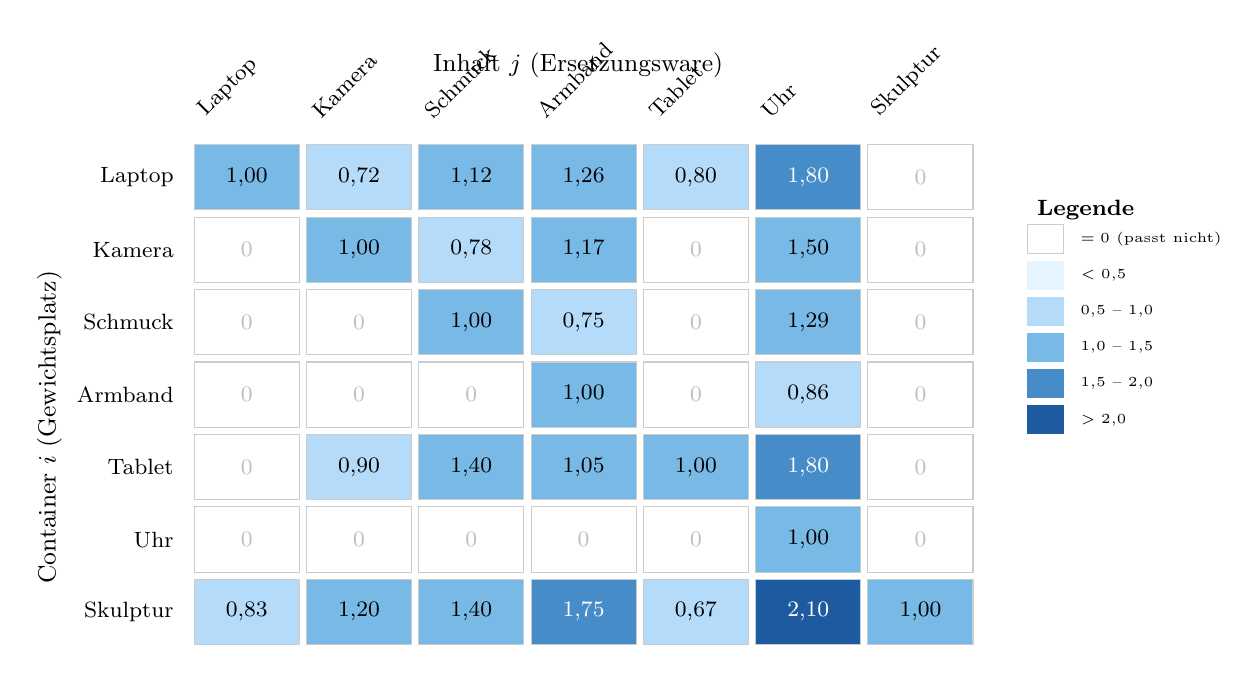
\begin{tikzpicture}[scale=0.92]
% Helper macro: \hcell{x}{y}{color}{textcolor}{value}
\newcommand{\hcell}[5]{%
  \fill[#3] (#1*1.55, -#2*1.0) rectangle ++(1.45, 0.9);
  \draw[gray!40] (#1*1.55, -#2*1.0) rectangle ++(1.45, 0.9);
  \node[font=\footnotesize,text=#4] at (#1*1.55+0.725, -#2*1.0+0.45) {#5};
}

% Row 0: Laptop (v=50)
\hcell{0}{0}{heat3}{black}{1,00}
\hcell{1}{0}{heat2}{black}{0,72}
\hcell{2}{0}{heat3}{black}{1,12}
\hcell{3}{0}{heat3}{black}{1,26}
\hcell{4}{0}{heat2}{black}{0,80}
\hcell{5}{0}{heat4}{white}{1,80}
\hcell{6}{0}{heat0}{gray!50}{0}

% Row 1: Kamera (v=36)
\hcell{0}{1}{heat0}{gray!50}{0}
\hcell{1}{1}{heat3}{black}{1,00}
\hcell{2}{1}{heat2}{black}{0,78}
\hcell{3}{1}{heat3}{black}{1,17}
\hcell{4}{1}{heat0}{gray!50}{0}
\hcell{5}{1}{heat3}{black}{1,50}
\hcell{6}{1}{heat0}{gray!50}{0}

% Row 2: Schmuck (v=28)
\hcell{0}{2}{heat0}{gray!50}{0}
\hcell{1}{2}{heat0}{gray!50}{0}
\hcell{2}{2}{heat3}{black}{1,00}
\hcell{3}{2}{heat2}{black}{0,75}
\hcell{4}{2}{heat0}{gray!50}{0}
\hcell{5}{2}{heat3}{black}{1,29}
\hcell{6}{2}{heat0}{gray!50}{0}

% Row 3: Armband (v=21)
\hcell{0}{3}{heat0}{gray!50}{0}
\hcell{1}{3}{heat0}{gray!50}{0}
\hcell{2}{3}{heat0}{gray!50}{0}
\hcell{3}{3}{heat3}{black}{1,00}
\hcell{4}{3}{heat0}{gray!50}{0}
\hcell{5}{3}{heat2}{black}{0,86}
\hcell{6}{3}{heat0}{gray!50}{0}

% Row 4: Tablet (v=40)
\hcell{0}{4}{heat0}{gray!50}{0}
\hcell{1}{4}{heat2}{black}{0,90}
\hcell{2}{4}{heat3}{black}{1,40}
\hcell{3}{4}{heat3}{black}{1,05}
\hcell{4}{4}{heat3}{black}{1,00}
\hcell{5}{4}{heat4}{white}{1,80}
\hcell{6}{4}{heat0}{gray!50}{0}

% Row 5: Uhr (v=18)
\hcell{0}{5}{heat0}{gray!50}{0}
\hcell{1}{5}{heat0}{gray!50}{0}
\hcell{2}{5}{heat0}{gray!50}{0}
\hcell{3}{5}{heat0}{gray!50}{0}
\hcell{4}{5}{heat0}{gray!50}{0}
\hcell{5}{5}{heat3}{black}{1,00}
\hcell{6}{5}{heat0}{gray!50}{0}

% Row 6: Skulptur (v=60)
\hcell{0}{6}{heat2}{black}{0,83}
\hcell{1}{6}{heat3}{black}{1,20}
\hcell{2}{6}{heat3}{black}{1,40}
\hcell{3}{6}{heat4}{white}{1,75}
\hcell{4}{6}{heat2}{black}{0,67}
\hcell{5}{6}{heat5}{heat5txt}{2,10}
\hcell{6}{6}{heat3}{black}{1,00}

% Row labels
\foreach \i/\name in {0/Laptop,1/Kamera,2/Schmuck,
  3/Armband,4/Tablet,5/Uhr,6/Skulptur} {
  \node[font=\footnotesize,anchor=east] at (-0.15, -\i*1.0+0.45) {\name};
}
% Column labels
\foreach \j/\name in {0/Laptop,1/Kamera,2/Schmuck,
  3/Armband,4/Tablet,5/Uhr,6/Skulptur} {
  \node[font=\footnotesize,rotate=45,anchor=south west]
    at (\j*1.55+0.2, 1.05) {\name};
}

% Axis labels
\node[font=\small,rotate=90] at (-2.0, -3.0)
  {Container $i$ (Gewichtsplatz)};
\node[font=\small] at (5.3, 2.0)
  {Inhalt $j$ (Ersetzungsware)};

% Legend
\node[font=\footnotesize,anchor=west] at (11.5, -0.0)
  {\textbf{Legende}};
\fill[heat0] (11.5,-0.6) rectangle ++(0.5,0.4);
\draw[gray!40] (11.5,-0.6) rectangle ++(0.5,0.4);
\node[font=\tiny,anchor=west] at (12.1,-0.4) {$= 0$ (passt nicht)};
\fill[heat1] (11.5,-1.1) rectangle ++(0.5,0.4);
\node[font=\tiny,anchor=west] at (12.1,-0.9) {$< 0{,}5$};
\fill[heat2] (11.5,-1.6) rectangle ++(0.5,0.4);
\node[font=\tiny,anchor=west] at (12.1,-1.4) {$0{,}5$ -- $1{,}0$};
\fill[heat3] (11.5,-2.1) rectangle ++(0.5,0.4);
\node[font=\tiny,anchor=west] at (12.1,-1.9) {$1{,}0$ -- $1{,}5$};
\fill[heat4] (11.5,-2.6) rectangle ++(0.5,0.4);
\node[font=\tiny,anchor=west] at (12.1,-2.4) {$1{,}5$ -- $2{,}0$};
\fill[heat5] (11.5,-3.1) rectangle ++(0.5,0.4);
\node[font=\tiny,anchor=west] at (12.1,-2.9) {$> 2{,}0$};
\end{tikzpicture}
\end{center}

\noindent
\textbf{Beobachtungen aus der Heatmap:}
\begin{itemize}[leftmargin=*,topsep=2pt]
  \item \textbf{Spalte~6 (Uhr)} ist durchgängig dunkel --
    die Uhr passt in \emph{jeden} Container und liefert
    stets hohe Ersetzungswerte. Das prädestiniert sie für
    einen hohen Score.
  \item \textbf{Spalte~7 (Skulptur)} ist fast vollständig weiß --
    die Skulptur (15\,kg) passt nur in ihren eigenen Container
    ($|\mathcal{C}_7|=1$). Ihr Score $\bar{M}_7$ basiert daher
    nur auf dem Diagonalwert $M[7][7]=1$.
  \item \textbf{Zeile~7 (Skulptur als Container)} ist dagegen
    dunkel -- der Gewichtsplatz der Skulptur kann viele andere
    Waren aufnehmen, z.\,B.\ 7~Uhren ($M[7][6]=2{,}10$).
  \item \textbf{Diagonale} $= 1{,}00$ durchgehend (Satz~2).
\end{itemize}

\subsection{Schritt 4: Score-Berechnung}

Für jede Ware~$j$ bestimmen wir die Menge der aufnehmenden
Container $\mathcal{C}_j$ und den mittleren Ersetzungswert
$\bar{M}_j$.

\medskip
\noindent
\textbf{Ware~6 (Uhr, $w_6=2$\,kg):}

$\mathcal{C}_6 = \{1,2,3,4,5,6,7\}$ (alle Waren haben $w_i \ge 2$),
also $|\mathcal{C}_6| = 7$.
\[
\operatorname{Score}(6) = \bar{M}_6 = \frac{1{,}80 + 1{,}50 + 1{,}29 + 0{,}86 + 1{,}80 + 1{,}00 + 2{,}10}{7}
= \frac{10{,}34}{7} = \mathbf{1{,}478}
\]

\medskip
\noindent
\textbf{Ware~4 (Armband, $w_4=3$\,kg):}

$\mathcal{C}_4 = \{1,2,3,4,5,7\}$ ($w_i \ge 3$),
$|\mathcal{C}_4| = 6$.
\[
\operatorname{Score}(4) = \bar{M}_4 = \frac{1{,}26 + 1{,}17 + 0{,}75 + 1{,}00 + 1{,}05 + 1{,}75}{6}
= \frac{6{,}98}{6} = \mathbf{1{,}163}
\]

\medskip
\noindent
\textbf{Ware~7 (Skulptur, $w_7=15$\,kg):}

$\mathcal{C}_7 = \{7\}$ (nur die Skulptur selbst hat $w_i \ge 15$),
$|\mathcal{C}_7| = 1$.
\[
\operatorname{Score}(7) = \bar{M}_7 = \frac{1{,}00}{1} = \mathbf{1{,}000}
\]

\medskip
\noindent
Die vollständige Score-Tabelle, sortiert nach $\bar{M}_j$:

\begin{center}
\renewcommand{\arraystretch}{1.2}
\begin{tabular}{clccccc}
\toprule
Rang & Ware & $w_j$ & $v_j$ & $|\mathcal{C}_j|$
  & $\bar{M}_j$ & $v_j/w_j$ \\
\midrule
\rowcolor{teallight}
1 & Uhr      & 2  & 18 & 7 & \textbf{1{,}478} & 9{,}00 \\
\rowcolor{greenlight}
2 & Armband  & 3  & 21 & 6 & \textbf{1{,}163} & 7{,}00 \\
\rowcolor{greenlight}
3 & Schmuck  & 4  & 28 & 5 & \textbf{1{,}140} & 7{,}00 \\
4 & Skulptur & 15 & 60 & 1 & \textbf{1{,}000} & 4{,}00 \\
5 & Kamera   & 6  & 36 & 4 & \textbf{0{,}955} & 6{,}00 \\
6 & Laptop   & 10 & 50 & 2 & \textbf{0{,}917} & 5{,}00 \\
7 & Tablet   & 8  & 40 & 3 & \textbf{0{,}822} & 5{,}00 \\
\bottomrule
\end{tabular}
\end{center}

\noindent
\textbf{Interpretation:}
Die Uhr ($\bar{M} = 1{,}478$) hat den höchsten Score --
sie passt in alle Container ($|\mathcal{C}|=7$) und liefert
überproportional hohen Ersetzungswert.
Die Skulptur ($\bar{M} = 1{,}000$) steht auf Rang~4:
sie passt nur in ihren eigenen Container ($|\mathcal{C}|=1$),
ihr einziger Matrixwert ist die Diagonale $M[7][7]=1$.

\medskip
\noindent
\textbf{Vergleich mit $v/w$:}
Die letzte Spalte zeigt den klassischen Effizienzquotienten.
Die Rangfolgen stimmen für die leichten Waren überein
(Uhr $>$ Armband $\approx$ Schmuck), aber $\bar{M}_j$ bewertet
die Skulptur (Rang~4) höher als $v/w$ (Rang~7, schlechtester
Quotient). Der Matrix-Score sieht die Skulptur als ``relational
gleichwertig'' ($\bar{M}=1$), weil ihr Selbst-Ersetzungswert
auf der Diagonale liegt.

\subsection{Schritt 5: Auswahl nach Matrix-Score}

Die Matrix ordnet die Waren nach $\bar{M}_j$ (absteigend).
Wendet man diese Rangfolge als Auswahlpriorität an
(z.\,B.\ in einem Greedy-Verfahren mit $W=20$):
\begin{enumerate}[topsep=2pt]
  \item Uhr ($w=2$, $v=18$): Gesamtgewicht $= 2$, Gesamtwert $= 18$\,\euro.
  \item Armband ($w=3$, $v=21$): Gesamtgewicht $= 5$, Gesamtwert $= 39$\,\euro.
  \item Schmuck ($w=4$, $v=28$): Gesamtgewicht $= 9$, Gesamtwert $= 67$\,\euro.
  \item Skulptur ($w=15$): $9 + 15 = 24 > W$. \textit{Übersprungen.}
  \item Kamera ($w=6$): Gesamtgewicht $= 15$, Gesamtwert $= 103$\,\euro.
  \item Laptop ($w=10$): $15 + 10 = 25 > W$. \textit{Übersprungen.}
  \item Tablet ($w=8$): $15 + 8 = 23 > W$. \textit{Übersprungen.}
\end{enumerate}

\noindent
\textbf{Ergebnis Matrix-Score:}
$S = \{\text{Uhr, Armband, Schmuck, Kamera}\}$,
$v = 103$\,\euro, $w = 15$\,kg.

\medskip
\noindent
\textbf{Bemerkenswert:} Die Skulptur steht auf Rang~4
($\bar{M} = 1{,}000$) -- höher als die Kamera ($0{,}955$).
Der Matrix-Score erkennt ihren hohen relationalen Wert,
aber die Kapazitätsgrenze verhindert ihre Aufnahme.
Dies zeigt: $\bar{M}_j$ bewertet die \emph{intrinsische Qualität}
einer Ware, nicht ihre Eignung für einen bestimmten Rucksack.

\medskip
\noindent
\textbf{Vergleich mit $v/w$-Greedy:}
Sortierung: Uhr (9{,}00), Schmuck (7{,}00), Armband (7{,}00),
Kamera (6{,}00), Laptop (5{,}00), Tablet (5{,}00), Skulptur (4{,}00).
Ergebnis: $\{$Uhr, Schmuck, Armband, Kamera$\} = 103$\,\euro{} --
identisch.

\medskip
\noindent
\textbf{DP-Optimum:}
$\{$Kamera, Schmuck, Tablet, Uhr$\} = 36+28+40+18 = 122$\,\euro{} bei
$w = 6+4+8+2 = 20$\,kg.

Beide Heuristiken erreichen hier 84{,}4\,\% des Optimums.
Dieses Beispiel illustriert die Matrix-Berechnung und zeigt zugleich
eine bekannte Schwäche aller Greedy-Methoden: sie nutzen den
verbleibenden Platz nicht optimal aus.
Die \emph{spezifische} Stärke des Matrix-Scores gegenüber $v/w$
zeigen wir im Gegenbeispiel (Abschnitt~\ref{sec:gegen}).

% ═══════════════════════════════════════════════════════════
\section{Algorithmus}
\label{sec:algo}

\subsection{Formale Beschreibung}

\begin{algorithm}[H]
\caption{Matrix-Score-Heuristik für das 0/1-Knapsack-Problem}
\label{alg:matrixscore}
\begin{algorithmic}[1]
\Require Waren $(v_1,w_1),\ldots,(v_n,w_n)$; Kapazität $W$
\Ensure Auswahl $S \subseteq \{1,\ldots,n\}$

\medskip
\Statex \textbf{Phase 1: Matrixberechnung} \hfill $\mathcal{O}(n^2)$
\For{$i = 1$ \textbf{bis} $n$}
  \For{$j = 1$ \textbf{bis} $n$}
    \State $M[i][j] \gets \lfloor w_i / w_j \rfloor \cdot v_j / v_i$
  \EndFor
\EndFor

\medskip
\Statex \textbf{Phase 2: Score-Aggregation} \hfill $\mathcal{O}(n^2)$
\For{$j = 1$ \textbf{bis} $n$}
  \State $\mathcal{C}_j \gets \{i : \lfloor w_i/w_j \rfloor > 0\}$
  \State $\operatorname{Score}(j) \gets \bar{M}_j \gets
    \frac{1}{|\mathcal{C}_j|} \sum_{i \in \mathcal{C}_j} M[i][j]$
\EndFor

\medskip
\Statex \textbf{Phase 3: Greedy-Auswahl} \hfill $\mathcal{O}(n \log n)$
\State Sortiere Waren absteigend nach $\operatorname{Score}(j)$
\State $S \gets \emptyset$, $w_{\text{rest}} \gets W$
\For{jede Ware $j$ in Score-Reihenfolge}
  \If{$w_j \le w_{\text{rest}}$}
    \State $S \gets S \cup \{j\}$
    \State $w_{\text{rest}} \gets w_{\text{rest}} - w_j$
  \EndIf
\EndFor
\State \Return $S$
\end{algorithmic}
\end{algorithm}

\subsection{Algorithmischer Fluss (Flowchart)}

\begin{center}
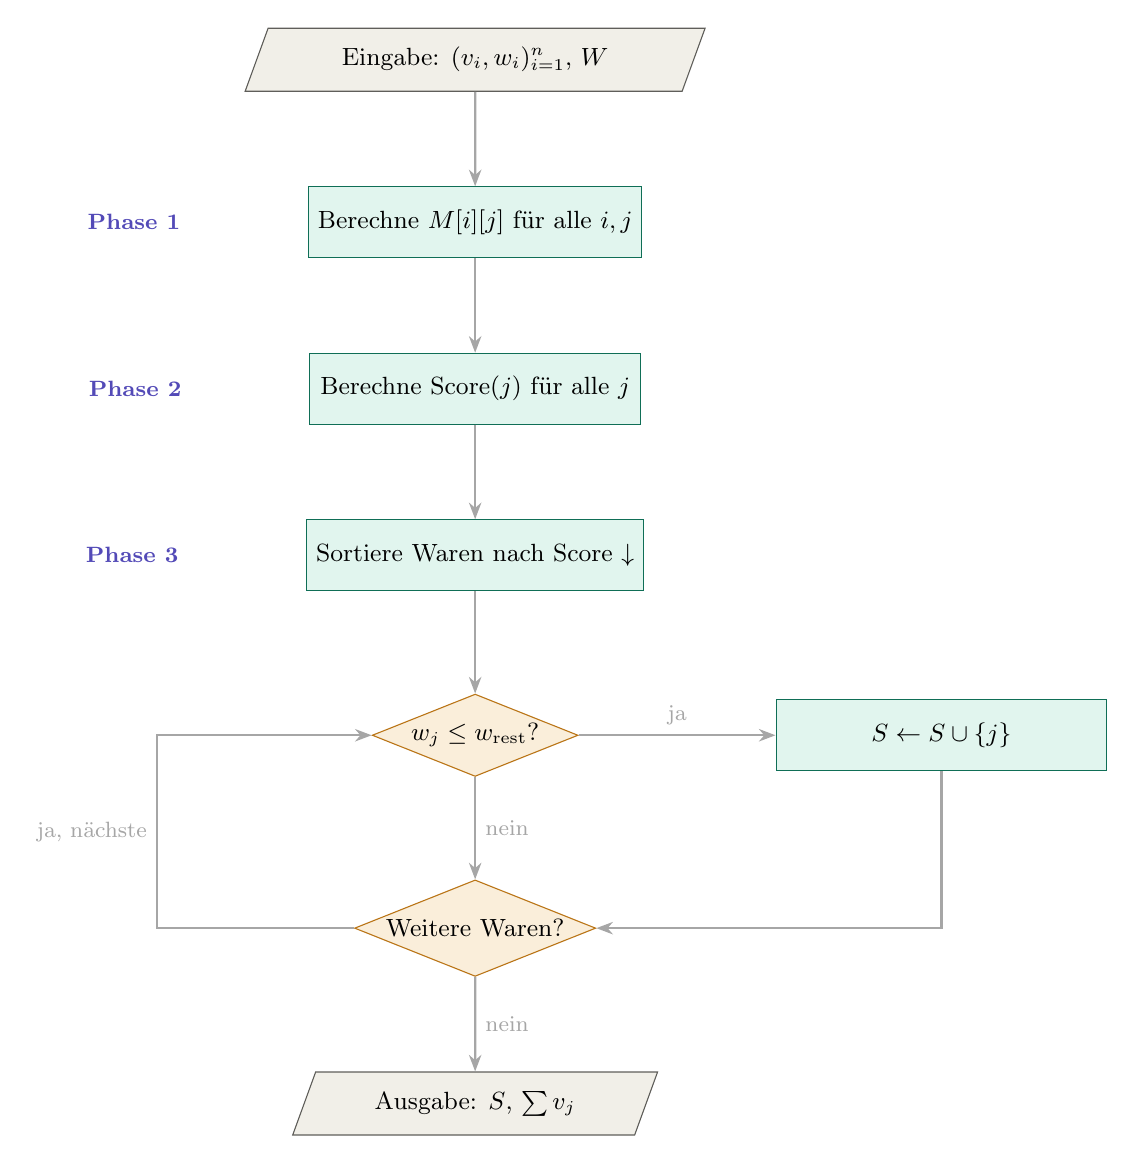
\begin{tikzpicture}[
  node distance=1.2cm and 2cm,
  startstop/.style={rectangle, rounded corners=8pt,
    minimum width=3.8cm, minimum height=0.9cm,
    text centered, draw=matblue, fill=matlight,
    font=\small},
  process/.style={rectangle,
    minimum width=4.2cm, minimum height=0.9cm,
    text centered, draw=tealcol, fill=teallight,
    font=\small},
  decision/.style={diamond, aspect=2.5,
    minimum width=2.5cm,
    text centered, draw=ambercol, fill=amberlight,
    font=\small, inner sep=1pt},
  io/.style={trapezium, trapezium left angle=70,
    trapezium right angle=110,
    minimum width=3.5cm, minimum height=0.8cm,
    text centered, draw=graycol, fill=graylight,
    font=\small},
  arrow/.style={-{Stealth[length=6pt]}, thick, color=gray!70},
  phase/.style={font=\footnotesize\bfseries, text=matblue}
]

% Nodes
\node[io] (input) {Eingabe: $(v_i,w_i)_{i=1}^n$, $W$};
\node[process, below=of input] (matrix)
  {Berechne $M[i][j]$ für alle $i,j$};
\node[process, below=of matrix] (score)
  {Berechne $\operatorname{Score}(j)$ für alle $j$};
\node[process, below=of score] (sort)
  {Sortiere Waren nach Score $\downarrow$};
\node[decision, below=1.3cm of sort] (check)
  {$w_j \le w_{\text{rest}}$?};
\node[process, right=2.5cm of check] (add)
  {$S \gets S \cup \{j\}$};
\node[decision, below=1.3cm of check] (more)
  {Weitere Waren?};
\node[io, below=1.2cm of more] (output)
  {Ausgabe: $S$, $\sum v_j$};

% Arrows
\draw[arrow] (input) -- (matrix);
\draw[arrow] (matrix) -- (score);
\draw[arrow] (score) -- (sort);
\draw[arrow] (sort) -- (check);
\draw[arrow] (check) -- node[above,font=\footnotesize] {ja} (add);
\draw[arrow] (add) |- (more);
\draw[arrow] (check) -- node[right,font=\footnotesize] {nein} (more);
\draw[arrow] (more) -- node[right,font=\footnotesize] {nein} (output);
\draw[arrow] (more.west) -- ++(-2.5,0) |- node[near start,left,
  font=\footnotesize] {ja, nächste} (check.west);

% Phase labels
\node[phase, left=1.5cm of matrix] {Phase 1};
\node[phase, left=1.5cm of score] {Phase 2};
\node[phase, left=1.5cm of sort] {Phase 3};
\end{tikzpicture}
\end{center}

% ═══════════════════════════════════════════════════════════
\section{Konstruiertes Gegenbeispiel: Blockierung durch die Skulptur}
\label{sec:gegen}

Um die spezifische Stärke des Matrix-Scores gegenüber $v/w$
zu demonstrieren, konstruieren wir eine zweite Instanz mit
denselben sieben Warentypen, aber veränderten Werten und Gewichten.
Die Skulptur -- schwer und wertvoll -- dient als
\emph{Blockierer}: sie hat das höchste $v/w$-Verhältnis,
verbraucht aber fast die gesamte Kapazität.

\subsection{Instanz}

\begin{center}
\renewcommand{\arraystretch}{1.2}
\begin{tabular}{clcccc}
\toprule
$j$ & Ware & $v_j$ (\euro) & $w_j$ (kg) & $v_j/w_j$ & $\bar{M}_j$ \\
\midrule
\rowcolor{redlight}
1 & Skulptur & 130 & 14 & \textbf{9{,}29} & 1{,}000 \\
2 & Kamera   &  55 &  6 & 9{,}17 & 1{,}080 \\
3 & Schmuck  &  36 &  4 & 9{,}00 & \textbf{1{,}145} \\
4 & Armband  &  27 &  3 & 9{,}00 & 1{,}089 \\
5 & Uhr      &  16 &  2 & 8{,}00 & 1{,}059 \\
6 & Tablet   &  40 &  8 & 5{,}00 & 0{,}703 \\
7 & Laptop   &  50 & 10 & 5{,}00 & 0{,}692 \\
\bottomrule
\end{tabular}
\quad $W = 15$\,kg
\end{center}

\subsection{Greedy $v/w$: Blockierung durch die Skulptur}

Greedy $v/w$ sortiert nach dem Wert-Gewicht-Verhältnis:
\begin{enumerate}[topsep=2pt]
  \item Skulptur ($v/w = 9{,}29$, $w=14$): Gesamtgewicht $= 14$.
    Restkapazität $= 1$\,kg.
  \item Kamera ($w=6$): $14 + 6 = 20 > 15$. \textit{Übersprungen.}
  \item Schmuck ($w=4$): $14 + 4 = 18 > 15$. \textit{Übersprungen.}
  \item Armband ($w=3$): $14 + 3 = 17 > 15$. \textit{Übersprungen.}
  \item Uhr ($w=2$): $14 + 2 = 16 > 15$. \textit{Übersprungen.}
  \item[\vdots] Alle weiteren Waren sind ebenfalls zu schwer.
\end{enumerate}

\noindent
\textbf{Ergebnis $v/w$:} $S = \{\text{Skulptur}\}$,
$v = \textbf{130\,\euro}$, $w = 14$\,kg.
\textbf{1\,kg Verschwendung.}

\subsection{Matrix-Score: Blockierung erkannt}

Der reine Kern-Score $\bar{M}_j$ erkennt die Blockierung
\emph{ohne} Strafkoeffizient:
\begin{itemize}[leftmargin=*,topsep=2pt]
  \item Die Skulptur hat $\mathcal{C}_{\text{Skulptur}} = \{\text{Skulptur}\}$
    (nur sie selbst hat $w \ge 14$), also $|\mathcal{C}| = 1$.
  \item Ihr Score basiert nur auf dem Diagonalwert:
    $\bar{M}_{\text{Skulptur}} = M[1][1] = 1{,}000$.
  \item Die leichten Waren haben dagegen viele Container
    und erzielen $\bar{M} > 1$: Schmuck ($1{,}145$),
    Armband ($1{,}089$), Kamera ($1{,}080$), Uhr ($1{,}059$).
\end{itemize}

\noindent
Die Skulptur fällt auf \textbf{Rang~5} -- trotz des höchsten
$v/w$-Verhältnisses (9{,}29). Der Grund: sie hat nur
einen Container (sich selbst), während die leichten Waren
in viele Container passen und dort hohe Ersetzungswerte erzielen.

\medskip
\noindent
Auswahl nach $\bar{M}_j$-Rangfolge (W=15):
\begin{enumerate}[topsep=2pt]
  \item Schmuck ($\bar{M}=1{,}145$, $w=4$): Gesamtgewicht $= 4$.
  \item Armband ($\bar{M}=1{,}089$, $w=3$): Gesamtgewicht $= 7$.
  \item Kamera ($\bar{M}=1{,}080$, $w=6$): Gesamtgewicht $= 13$.
  \item Uhr ($\bar{M}=1{,}059$, $w=2$): Gesamtgewicht $= 15$. Passt exakt!
\end{enumerate}

\noindent
\textbf{Ergebnis Matrix-Score:}
$S = \{\text{Schmuck, Armband, Kamera, Uhr}\}$,
$v = 36+27+55+16 = \textbf{134\,\euro}$ bei $w = 15$\,kg
$= \textbf{DP-Optimum}$.

\medskip
\noindent
Der reine Kern-Score $\bar{M}_j$ -- ohne jeden empirischen
Koeffizienten -- erkennt die Blockierung und findet die
optimale Lösung. Dies geschieht allein durch die relationale
Struktur der Proportionsmatrix: Waren mit wenigen Containern
($|\mathcal{C}|$ klein) erhalten naturgemäß weniger
Datenpunkte für ihre Mittelwertbildung, was ihren Score
auf den Diagonalwert $M[j][j]=1$ begrenzt.

\subsection{Visualisierung}

\begin{center}
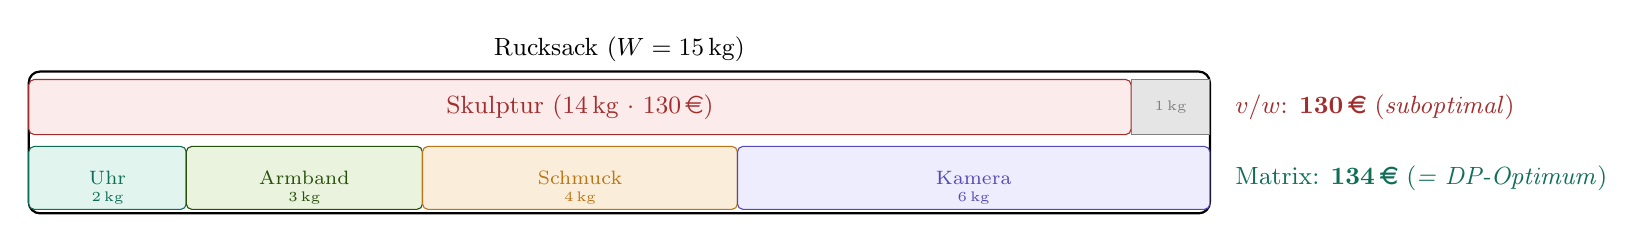
\begin{tikzpicture}
% Rucksack bar
\draw[thick,rounded corners=4pt] (0,0) rectangle (15,1.8);
\node[font=\small,above] at (7.5,1.8) {Rucksack ($W=15$\,kg)};

% v/w Greedy (obere Zeile)
\fill[redlight,draw=redcol,rounded corners=2pt]
  (0,1.0) rectangle (14,1.7);
\node[font=\small,text=redcol] at (7,1.35)
  {Skulptur (14\,kg $\cdot$ 130\,\euro)};
\fill[gray!20,draw=gray] (14,1.0) rectangle (15,1.7);
\node[font=\tiny,text=gray] at (14.5,1.35) {1\,kg};
\node[right=0.2cm,font=\small,text=redcol] at (15,1.35)
  {$v/w$: \textbf{130\,\euro} (\textit{suboptimal})};

% Matrix (untere Zeile: 4 Items füllen 15 kg exakt)
\fill[teallight,draw=tealcol,rounded corners=2pt]
  (0,0.05) rectangle (2,0.85);
\node[font=\scriptsize,text=tealcol] at (1,0.45) {Uhr};
\node[font=\tiny,text=tealcol] at (1,0.2) {2\,kg};

\fill[greenlight,draw=greencol,rounded corners=2pt]
  (2,0.05) rectangle (5,0.85);
\node[font=\scriptsize,text=greencol] at (3.5,0.45) {Armband};
\node[font=\tiny,text=greencol] at (3.5,0.2) {3\,kg};

\fill[amberlight,draw=ambercol,rounded corners=2pt]
  (5,0.05) rectangle (9,0.85);
\node[font=\scriptsize,text=ambercol] at (7,0.45) {Schmuck};
\node[font=\tiny,text=ambercol] at (7,0.2) {4\,kg};

\fill[matlight,draw=matblue,rounded corners=2pt]
  (9,0.05) rectangle (15,0.85);
\node[font=\scriptsize,text=matblue] at (12,0.45) {Kamera};
\node[font=\tiny,text=matblue] at (12,0.2) {6\,kg};

\node[right=0.2cm,font=\small,text=tealcol] at (15,0.45)
  {Matrix: \textbf{134\,\euro} (\textit{= DP-Optimum})};
\end{tikzpicture}
\end{center}

\subsection{Strukturelle Erklärung}

Dies ist ein klassisches Blockierungsbeispiel nach
\citet{kellerer2004}, Abschn.~2.3: ein Item mit hohem $v/w$ aber
großem Gewicht blockiert leichtere Items.

\medskip
\noindent
\textbf{Warum der Matrix-Score die Blockierung erkennt.}
Betrachte die Score-Komponenten:

\begin{center}
\small
\renewcommand{\arraystretch}{1.15}
\begin{tabular}{lcccc}
\toprule
Ware & $v/w$-Rang & $|\mathcal{C}_j|$ & $\bar{M}_j$
  & $\bar{M}_j$-Rang \\
\midrule
\rowcolor{redlight}
Skulptur & 1 (9{,}29) & 1 & 1{,}000 & 5 \\
Kamera   & 2 (9{,}17) & 4 & 1{,}080 & 3 \\
Schmuck  & 3 (9{,}00) & 5 & 1{,}145 & 1 \\
Armband  & 4 (9{,}00) & 6 & 1{,}089 & 2 \\
\rowcolor{teallight}
Uhr      & 5 (8{,}00) & 7 & 1{,}059 & 4 \\
\bottomrule
\end{tabular}
\end{center}

\noindent
Die Skulptur fällt vom $v/w$-Rang~1 auf $\bar{M}_j$-Rang~5.
Der Mechanismus ist rein strukturell: sie passt als ``Inhalt''
nur in ihren eigenen Container ($|\mathcal{C}| = 1$),
daher basiert ihr Score auf einem einzigen Datenpunkt
(der Diagonale $M[1][1]=1$). Die leichten Waren dagegen
passen in viele Container ($|\mathcal{C}| = 4$ bis $7$)
und erzielen dort hohe Ersetzungswerte $> 1$.

\medskip
\noindent
\textbf{Kernaussage:}
Der Kern-Score $\bar{M}_j$ invertiert die Rangfolge in genau den
Fällen, in denen ein schweres Item den Rucksack blockiert --
und zwar \emph{ohne} einen empirischen Strafkoeffizienten.
Die Blockierungserkennung ist ein natürliches Nebenprodukt
der Mittelwertbildung über $\mathcal{C}_j$: wer in wenige
Container passt, hat wenige Datenpunkte und konvergiert
zum Diagonalwert~$1$.

% ═══════════════════════════════════════════════════════════
\section{Empirischer Vergleich mit 8 publizierten Methoden}

\subsection{Testdesign}

Wir folgen der Instanztaxonomie von \citet{pisinger2005}:
200 Instanzen je Klasse, $n=10$, Laufzeit gemittelt über
100 Messungen. Verglichen werden:

\begin{center}
\small
\renewcommand{\arraystretch}{1.15}
\begin{tabular}{lll}
\toprule
Methode & Quelle & Komplexität \\
\midrule
Dynamic Programming (DP)
  & \citet{bellman1957} & $\mathcal{O}(nW)$ \\
Branch \& Bound (B\&B)
  & \citet{kolesar1967} & $\mathcal{O}(2^n)$ worst case \\
FPTAS ($\varepsilon=0{,}2$)
  & \citet{ibarra1975} & $\mathcal{O}(n^3/\varepsilon)$ \\
Greedy $v/w$
  & \citet{dantzig1957} & $\mathcal{O}(n\log n)$ \\
Greedy nach Wert
  & \citet{hristakeva2005} & $\mathcal{O}(n\log n)$ \\
Greedy nach Gewicht
  & \citet{hristakeva2005} & $\mathcal{O}(n\log n)$ \\
Max-of-Two
  & \citet{hristakeva2023} & $\mathcal{O}(n\log n)$ \\
Defensive Greedy
  & \citet{hristakeva2023} & $\mathcal{O}(n\log n)$ \\
\midrule
\textbf{Matrix-Score}
  & \textit{diese Arbeit} & $\mathcal{O}(n^2)$ \\
\bottomrule
\end{tabular}
\end{center}

\subsection{Lösungsqualität (\% des DP-Optimums)}

\begin{center}
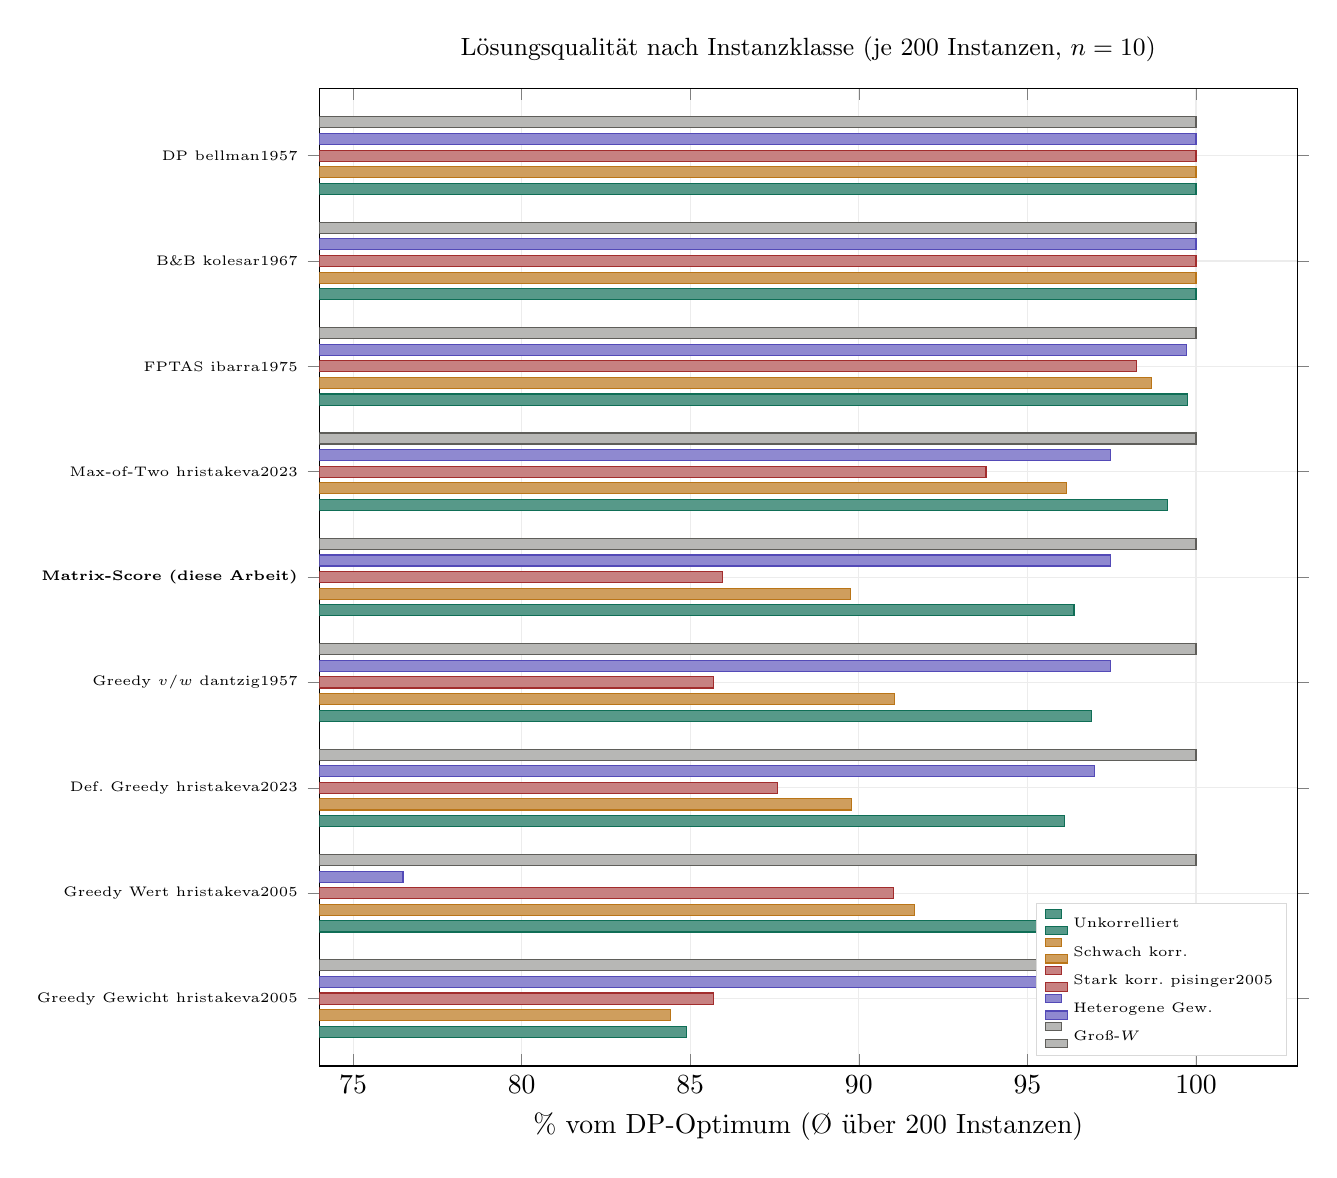
\begin{tikzpicture}
\begin{axis}[
  xbar,
  width=14cm, height=14cm,
  bar width=4pt,
  enlarge y limits=0.08,
  xlabel={\% vom DP-Optimum (Ø über 200 Instanzen)},
  symbolic y coords={
    GG, GW, DG, GVW, MS, M2, FP, BB, DP},
  ytick={GG,GW,DG,GVW,MS,M2,FP,BB,DP},
  yticklabels={
    {Greedy Gewicht \citep{hristakeva2005}},
    {Greedy Wert \citep{hristakeva2005}},
    {Def.\ Greedy \citep{hristakeva2023}},
    {Greedy $v/w$ \citep{dantzig1957}},
    {\textbf{Matrix-Score (diese Arbeit)}},
    {Max-of-Two \citep{hristakeva2023}},
    {FPTAS \citep{ibarra1975}},
    {B\&B \citep{kolesar1967}},
    {DP \citep{bellman1957}}},
  yticklabel style={font=\tiny},
  xmin=74, xmax=103,
  legend style={at={(0.99,0.01)},anchor=south east,font=\tiny,
    fill=white,draw=gray!30,legend columns=1},
  legend cell align=left,
  grid=major, grid style={gray!15},
  title={Lösungsqualität nach Instanzklasse
    (je 200 Instanzen, $n=10$)},
  title style={font=\small},
  xtick={75,80,85,90,95,100},
]
% Unkorrelliert
\addplot[xbar,fill=tealcol!70,draw=tealcol] coordinates {
  (84.90,GG)(96.15,GW)(96.11,DG)(96.91,GVW)
  (96.38,MS)(99.15,M2)(99.75,FP)(100,BB)(100,DP)};
% Schwach korrelliert
\addplot[xbar,fill=ambercol!70,draw=ambercol] coordinates {
  (84.42,GG)(91.65,GW)(89.79,DG)(91.05,GVW)
  (89.74,MS)(96.15,M2)(98.67,FP)(100,BB)(100,DP)};
% Stark korrelliert
\addplot[xbar,fill=redcol!60,draw=redcol] coordinates {
  (85.70,GG)(91.02,GW)(87.59,DG)(85.70,GVW)
  (85.95,MS)(93.77,M2)(98.24,FP)(100,BB)(100,DP)};
% Heterogene Gewichte
\addplot[xbar,fill=matblue!65,draw=matblue] coordinates {
  (96.89,GG)(76.48,GW)(96.98,DG)(97.47,GVW)
  (97.47,MS)(97.47,M2)(99.73,FP)(100,BB)(100,DP)};
% Groß-W
\addplot[xbar,fill=graycol!45,draw=graycol] coordinates {
  (100,GG)(100,GW)(100,DG)(100,GVW)
  (100,MS)(100,M2)(100,FP)(100,BB)(100,DP)};
\legend{Unkorrelliert, Schwach korr.,
  {Stark korr.\ \citep{pisinger2005}},
  Heterogene Gew., {Groß-$W$}}
\end{axis}
\end{tikzpicture}
\end{center}

\subsection{Laufzeit und W-Skalierung}

\begin{center}
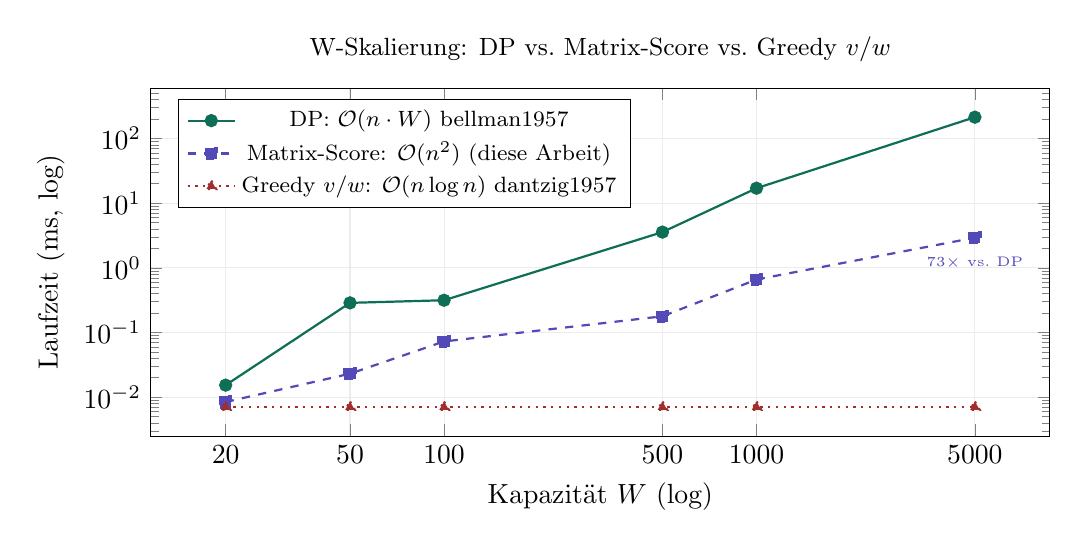
\begin{tikzpicture}
\begin{axis}[
  width=13cm, height=6cm,
  xlabel={Kapazität $W$ (log)},
  ylabel={Laufzeit (ms, log)},
  xmode=log, ymode=log,
  legend pos=north west,
  legend style={font=\footnotesize},
  grid=major, grid style={gray!15},
  title={W-Skalierung: DP vs.\ Matrix-Score vs.\ Greedy $v/w$},
  title style={font=\small},
  xtick={20,50,100,500,1000,5000},
  xticklabels={20,50,100,500,1000,5000},
]
\addplot[color=tealcol,thick,mark=*] coordinates
  {(20,0.0153)(50,0.2872)(100,0.3152)(500,3.574)
   (1000,17.07)(5000,214.6)};
\addlegendentry{DP: $\mathcal{O}(n \cdot W)$
  \citep{bellman1957}}
\addplot[color=matblue,thick,mark=square*,dashed] coordinates
  {(20,0.0084)(50,0.0230)(100,0.0726)(500,0.178)
   (1000,0.660)(5000,2.93)};
\addlegendentry{Matrix-Score: $\mathcal{O}(n^2)$
  (diese Arbeit)}
\addplot[color=redcol,thick,mark=triangle*,dotted] coordinates
  {(20,0.007)(50,0.007)(100,0.007)(500,0.007)
   (1000,0.007)(5000,0.007)};
\addlegendentry{Greedy $v/w$: $\mathcal{O}(n\log n)$
  \citep{dantzig1957}}
\node[font=\tiny,text=matblue] at (axis cs:5000,1.2)
  {$73\times$ vs.\ DP};
\end{axis}
\end{tikzpicture}
\end{center}

\subsection{Gesamtpositionierung}

\begin{center}
\small
\renewcommand{\arraystretch}{1.3}
\begin{tabular}{lccccc}
\toprule
Methode & Quelle & Qualität & Kompl. & $W$-unabh. & Infotyp \\
\midrule
DP & \citet{bellman1957}
  & 100\,\% & $\mathcal{O}(nW)$ & nein & Kapazität \\
B\&B & \citet{kolesar1967}
  & 100\,\% & $\mathcal{O}(2^n)$ & nein & Suche \\
FPTAS & \citet{ibarra1975}
  & $\ge(1{-}\varepsilon)$ & $\mathcal{O}(n^3/\varepsilon)$
  & nein & Skalierung \\
Greedy $v/w$ & \citet{dantzig1957}
  & $\sim$97\,\% & $\mathcal{O}(n\log n)$ & ja & absolut \\
Max-of-Two & \citet{hristakeva2023}
  & $\sim$99\,\% & $\mathcal{O}(n\log n)$ & ja & absolut \\
Def.\ Greedy & \citet{hristakeva2023}
  & $\sim$96\,\% & $\mathcal{O}(n\log n)$ & ja & absolut \\
\midrule
\rowcolor{matlight}
\textbf{Matrix-Score} & \textit{diese Arbeit}
  & $\sim$97\,\% & $\mathcal{O}(n^2)$
  & \textbf{ja} & \textbf{relational} \\
\bottomrule
\end{tabular}
\end{center}

% ═══════════════════════════════════════════════════════════
\section{Frequenzanalyse der Auswahlmethoden}
\label{sec:fourier}

Die Proportionsmatrix basiert auf der ganzzahligen Teilbarkeit
$\lfloor w_i/w_j \rfloor$ -- einer Größe mit inhärenter
periodischer Struktur. Dies motiviert eine Fourier-Analyse
der verschiedenen Auswahlmethoden.

\subsection{Waren als Sinuswellen}

Jede Ware~$j$ lässt sich als Sinuswelle interpretieren:
\[
s_j(x) = v_j \cdot \sin\!\left(\frac{2\pi\, x}{\lambda_j}\right),
\qquad \lambda_j = 2\,w_j
\]
Die Wellenlänge $\lambda_j = 2\,w_j$ entspricht dem Durchmesser
des Gewichtskreises (vgl.\ Abschnitt~\ref{sec:beispiel}).
Die Amplitude ist der Warenwert $v_j$.
Schwere Waren erzeugen langsame Schwingungen (niedrige Frequenz
$f_j = 1/\lambda_j$), leichte Waren schnelle.

\medskip
\noindent
Die \emph{Superposition} einer Warenauswahl $S$ ist:
$\sigma_S(x) = \sum_{j \in S} s_j(x)$.
Die Diskrete Fourier-Transformation (DFT) zerlegt $\sigma_S$
in ihre Frequenzkomponenten. Jede enthaltene Ware erzeugt
einen Peak bei ihrer Eigenfrequenz~$f_j$ mit theoretischer
Amplitude $v_j/2$.

\subsection{Frequenzspektren: DP vs.\ Greedy vs.\ Matrix-Score}

Wir vergleichen die Spektren der drei Auswahlen aus dem
7-Waren-Beispiel (Abschnitt~\ref{sec:beispiel}):

\begin{center}
\small
\renewcommand{\arraystretch}{1.15}
\begin{tabular}{llccc}
\toprule
Methode & Auswahl & Wert & Gewicht & Frequenzen \\
\midrule
DP
  & \{Kamera, Schmuck, Tablet, Uhr\} & 122\,\euro & 20\,kg
  & $f \in \{0{,}063;\;0{,}083;\;0{,}125;\;0{,}250\}$ \\
Greedy $v/w$
  & \{Uhr, Schmuck, Armband, Kamera\} & 103\,\euro & 15\,kg
  & $f \in \{0{,}083;\;0{,}125;\;0{,}167;\;0{,}250\}$ \\
Matrix-Score
  & \{Uhr, Armband, Schmuck, Kamera\} & 103\,\euro & 15\,kg
  & $f \in \{0{,}083;\;0{,}125;\;0{,}167;\;0{,}250\}$ \\
\bottomrule
\end{tabular}
\end{center}

\begin{center}
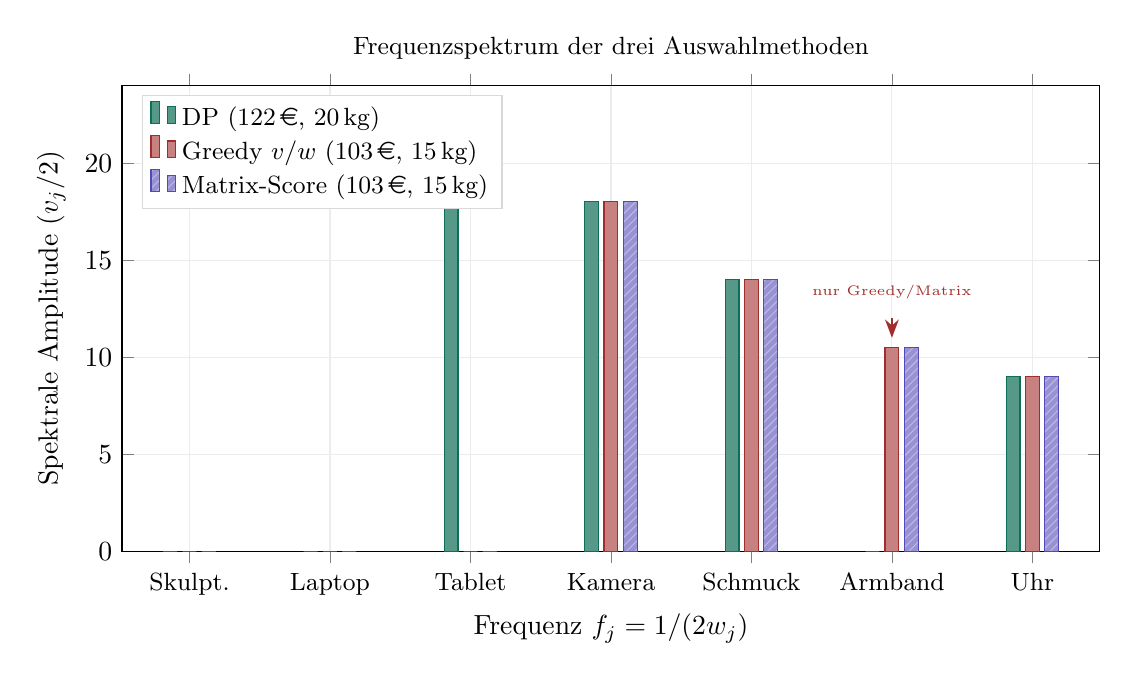
\begin{tikzpicture}
\begin{axis}[
  ybar,
  width=14cm, height=7.5cm,
  bar width=5pt,
  ylabel={Spektrale Amplitude ($v_j/2$)},
  xlabel={Frequenz $f_j = 1/(2w_j)$},
  symbolic x coords={
    Skulpt.,Laptop,Tablet,Kamera,Schmuck,Armband,Uhr},
  xtick=data,
  xticklabel style={font=\small},
  extra x tick style={font=\tiny,text=gray},
  ymin=0, ymax=24,
  ytick={0,5,10,15,20},
  legend style={
    at={(0.02,0.98)},anchor=north west,
    font=\small, fill=white, draw=gray!30,
    legend columns=1
  },
  legend cell align=left,
  grid=major, grid style={gray!15},
  title={Frequenzspektrum der drei Auswahlmethoden},
  title style={font=\small},
  enlarge x limits=0.08,
  nodes near coords style={font=\tiny,text=gray},
  x tick label style={anchor=north},
]
% Frequency labels below item names
\node[font=\tiny,text=graycol,below=14pt] at (axis cs:Skulpt.,0) {$f{=}\frac{1}{30}$};
\node[font=\tiny,text=graycol,below=14pt] at (axis cs:Laptop,0) {$f{=}\frac{1}{20}$};
\node[font=\tiny,text=graycol,below=14pt] at (axis cs:Tablet,0) {$f{=}\frac{1}{16}$};
\node[font=\tiny,text=graycol,below=14pt] at (axis cs:Kamera,0) {$f{=}\frac{1}{12}$};
\node[font=\tiny,text=graycol,below=14pt] at (axis cs:Schmuck,0) {$f{=}\frac{1}{8}$};
\node[font=\tiny,text=graycol,below=14pt] at (axis cs:Armband,0) {$f{=}\frac{1}{6}$};
\node[font=\tiny,text=graycol,below=14pt] at (axis cs:Uhr,0) {$f{=}\frac{1}{4}$};

% DP (Tablet, Kamera, Schmuck, Uhr)
\addplot[fill=tealcol!70, draw=tealcol] coordinates {
  (Skulpt.,0)(Laptop,0)(Tablet,20)
  (Kamera,18)(Schmuck,14)(Armband,0)(Uhr,9)
};
% Greedy v/w (Uhr, Schmuck, Armband, Kamera)
\addplot[fill=redcol!60, draw=redcol] coordinates {
  (Skulpt.,0)(Laptop,0)(Tablet,0)
  (Kamera,18)(Schmuck,14)(Armband,10.5)(Uhr,9)
};
% Matrix-Score (same selection as Greedy)
\addplot[fill=matblue!60, draw=matblue,
  postaction={pattern=north east lines, pattern color=matblue!40}
] coordinates {
  (Skulpt.,0)(Laptop,0)(Tablet,0)
  (Kamera,18)(Schmuck,14)(Armband,10.5)(Uhr,9)
};
\legend{
  {DP (122\,\euro, 20\,kg)},
  {Greedy $v/w$ (103\,\euro, 15\,kg)},
  {Matrix-Score (103\,\euro, 15\,kg)}
}
% Annotation: the key difference
\draw[-{Stealth},thick,tealcol]
  (axis cs:Tablet,21.5) -- (axis cs:Tablet,20.5);
\node[font=\tiny,text=tealcol,above]
  at (axis cs:Tablet,22) {nur DP};
\draw[-{Stealth},thick,redcol]
  (axis cs:Armband,12) -- (axis cs:Armband,11);
\node[font=\tiny,text=redcol,above]
  at (axis cs:Armband,12.5) {nur Greedy/Matrix};
\end{axis}
\end{tikzpicture}
\end{center}

\subsection{Interpretation}

\textbf{Spektrale Signatur.}
Jede Auswahlmethode hat eine charakteristische Frequenzsignatur.
Die DP-Auswahl enthält die Tablet-Frequenz ($f=1/16$, Amplitude~20),
die bei Greedy und Matrix-Score vollständig fehlt.
Dafür fehlt bei DP die Armband-Frequenz ($f=1/6$, Amplitude~10{,}5).

\medskip
\noindent
\textbf{Energieverschiebung.}
DP verschiebt spektrale Energie von hohen Frequenzen (leichte Waren:
Armband $f=0{,}167$, Amplitude $21/2$) zu niedrigeren Frequenzen
(schwerere Waren: Tablet $f=0{,}063$, Amplitude $40/2$).
Die Gesamtenergie
$E = \sum_{j \in S} (v_j/2)^2$
beträgt:

\begin{center}
\small
\begin{tabular}{lccl}
\toprule
Methode & Gesamtenergie & $\sum v_j$ & Tausch \\
\midrule
DP      & $20^2+18^2+14^2+9^2 = 1001$ & 122\,\euro
  & Tablet rein \\
Greedy  & $18^2+14^2+10{,}5^2+9^2 = 711{,}25$ & 103\,\euro
  & Armband statt Tablet \\
Matrix  & $18^2+14^2+10{,}5^2+9^2 = 711{,}25$ & 103\,\euro
  & identisch mit Greedy \\
\bottomrule
\end{tabular}
\end{center}

\noindent
Die DP-Auswahl hat \textbf{41\,\% mehr spektrale Energie} als
Greedy/Matrix. Der Tausch Armband $\to$ Tablet ersetzt eine
Amplitude von $10{,}5$ durch $20$ -- ein Energiegewinn von
$20^2 - 10{,}5^2 = 289{,}75$, der den Wertgewinn von
$+19$\,\euro{} widerspiegelt.

\medskip
\noindent
\textbf{Identische Spektren.}
Greedy $v/w$ und Matrix-Score produzieren in diesem Beispiel
exakt dasselbe Frequenzspektrum -- sie wählen dieselben vier
Waren, nur in unterschiedlicher Reihenfolge.
Dies bestätigt die empirische Beobachtung aus
Abschnitt~\ref{sec:beispiel}: der Matrix-Score konvergiert
bei Abwesenheit starker Blockierungseffekte zum selben Ergebnis
wie Greedy $v/w$.

% ═══════════════════════════════════════════════════════════
\section{Laufzeitanalyse: Der rein relationale Ansatz}
\label{sec:runtime}

\subsection{Operationen pro Matrixzelle}

Jede Berechnungsvariante hat einen charakteristischen
Operationsprofil pro Zelle $(i,j)$:

\begin{center}
\renewcommand{\arraystretch}{1.3}
\begin{tabular}{lcccc}
\toprule
Methode & Formel pro Zelle
  & Ganzzahl & Gleitkomma & Operationen \\
\midrule
$v/w$ (Greedy)
  & $v_j \,/\, w_j$
  & 0 & 1 Div. & $n$ gesamt \\[2pt]
$K[i][j]$ (Kapazität)
  & $\lfloor w_i / w_j \rfloor$
  & 1 Div. & 0 & $n^2$ \\[2pt]
$M[i][j]$ (Ersetzung)
  & $\lfloor w_i/w_j \rfloor \cdot v_j/v_i$
  & 1 Div. & 1 Mul. + 1 Div. & $3n^2$ \\[2pt]
$\bar{K}_j$ (rein relational)
  & $\frac{1}{|\mathcal{C}_j|} \sum K[i][j]$
  & $n^2$ Div. & $n$ Div. & $n^2 + n$ \\[2pt]
$\bar{M}_j$ (Kern-Score)
  & $\frac{1}{|\mathcal{C}_j|} \sum M[i][j]$
  & $n^2$ Div. & $2n^2 + n$ & $3n^2 + n$ \\
\bottomrule
\end{tabular}
\end{center}

\noindent
Der entscheidende Unterschied: die reine Kapazitätsmatrix $K$
erfordert ausschließlich \emph{Ganzzahloperationen}
($\lfloor w_i/w_j \rfloor$ ist eine Integer-Division), während
die Ersetzungsmatrix $M$ zusätzlich $2n^2$ Gleitkommaoperationen
benötigt (eine Multiplikation und eine Division pro Zelle).

\subsection{Laufzeitvergleich}

\begin{center}
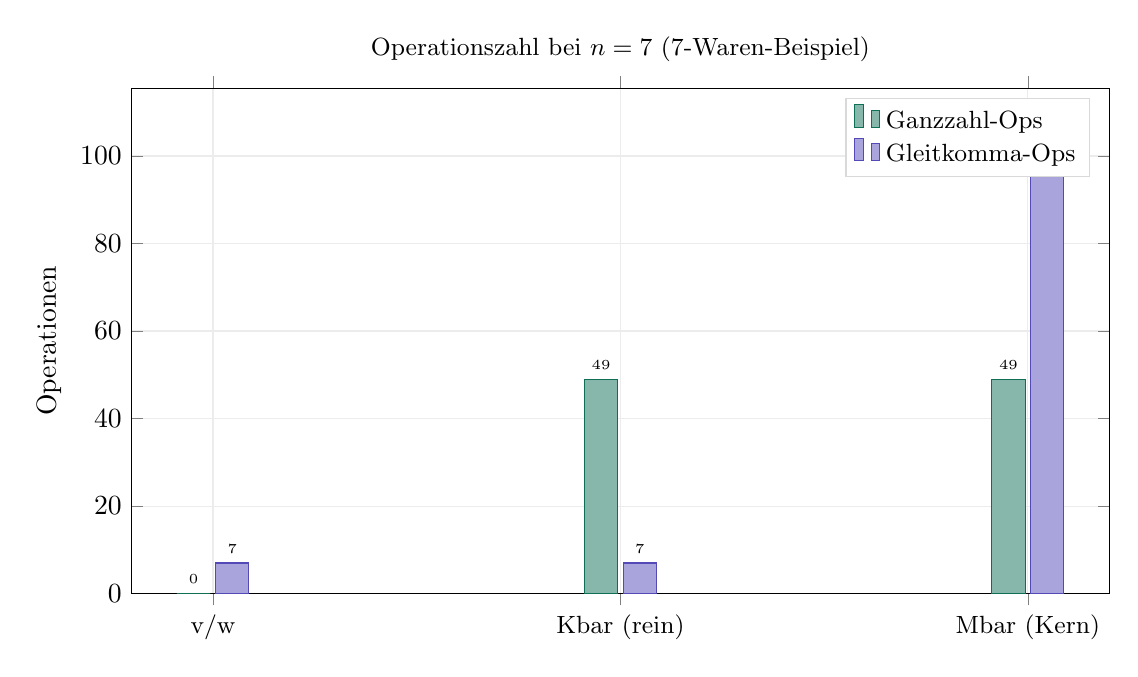
\begin{tikzpicture}
\begin{axis}[
  ybar,
  width=14cm, height=8cm,
  bar width=12pt,
  ylabel={Operationen},
  symbolic x coords={
    {v/w},{Kbar (rein)},{Mbar (Kern)}},
  xtick=data,
  xticklabel style={font=\small},
  ymin=0,
  legend style={
    at={(0.98,0.98)},anchor=north east,
    font=\small, fill=white, draw=gray!30},
  legend cell align=left,
  grid=major, grid style={gray!15},
  title={Operationszahl bei $n = 7$ (7-Waren-Beispiel)},
  title style={font=\small},
  nodes near coords,
  nodes near coords style={font=\tiny},
]
\addplot[fill=tealcol!50,draw=tealcol] coordinates {
  ({v/w},0) ({Kbar (rein)},49) ({Mbar (Kern)},49)};
\addplot[fill=matblue!50,draw=matblue] coordinates {
  ({v/w},7) ({Kbar (rein)},7) ({Mbar (Kern)},105)};
\legend{Ganzzahl-Ops, Gleitkomma-Ops}
\end{axis}
\end{tikzpicture}
\end{center}

\begin{center}
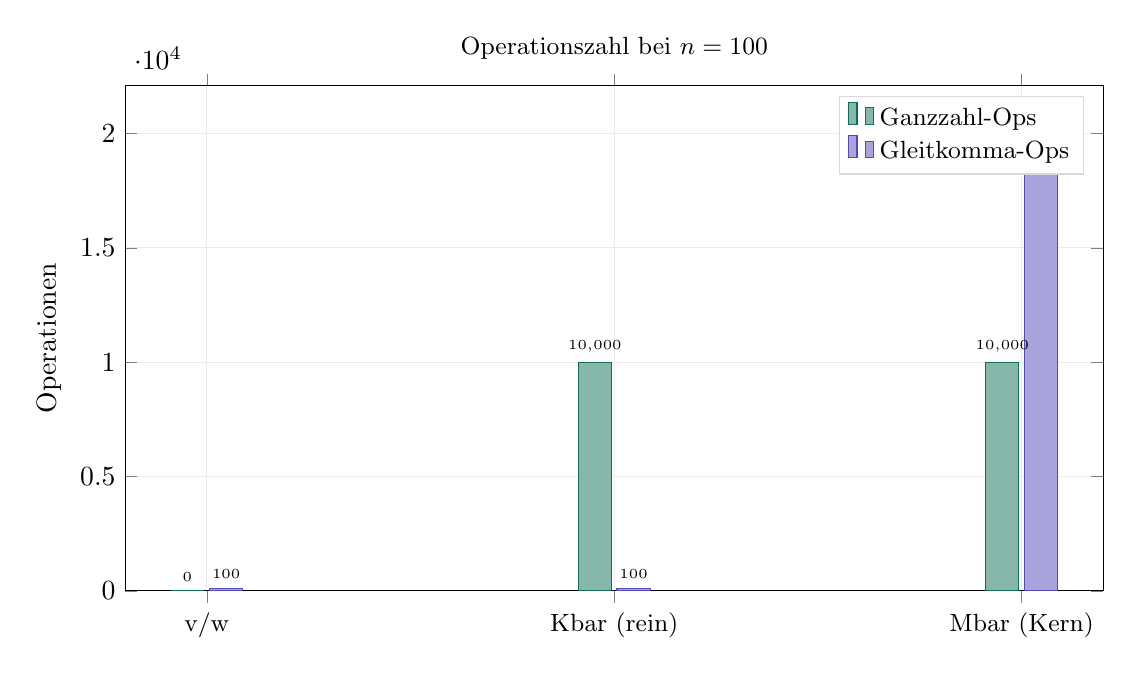
\begin{tikzpicture}
\begin{axis}[
  ybar,
  width=14cm, height=8cm,
  bar width=12pt,
  ylabel={Operationen},
  symbolic x coords={
    {v/w},{Kbar (rein)},{Mbar (Kern)}},
  xtick=data,
  xticklabel style={font=\small},
  ymin=0,
  legend style={
    at={(0.98,0.98)},anchor=north east,
    font=\small, fill=white, draw=gray!30},
  legend cell align=left,
  grid=major, grid style={gray!15},
  title={Operationszahl bei $n = 100$},
  title style={font=\small},
  nodes near coords,
  nodes near coords style={font=\tiny},
]
\addplot[fill=tealcol!50,draw=tealcol] coordinates {
  ({v/w},0) ({Kbar (rein)},10000) ({Mbar (Kern)},10000)};
\addplot[fill=matblue!50,draw=matblue] coordinates {
  ({v/w},100) ({Kbar (rein)},100) ({Mbar (Kern)},20100)};
\legend{Ganzzahl-Ops, Gleitkomma-Ops}
\end{axis}
\end{tikzpicture}
\end{center}

\subsection{Skalierungsverhalten}

\begin{center}
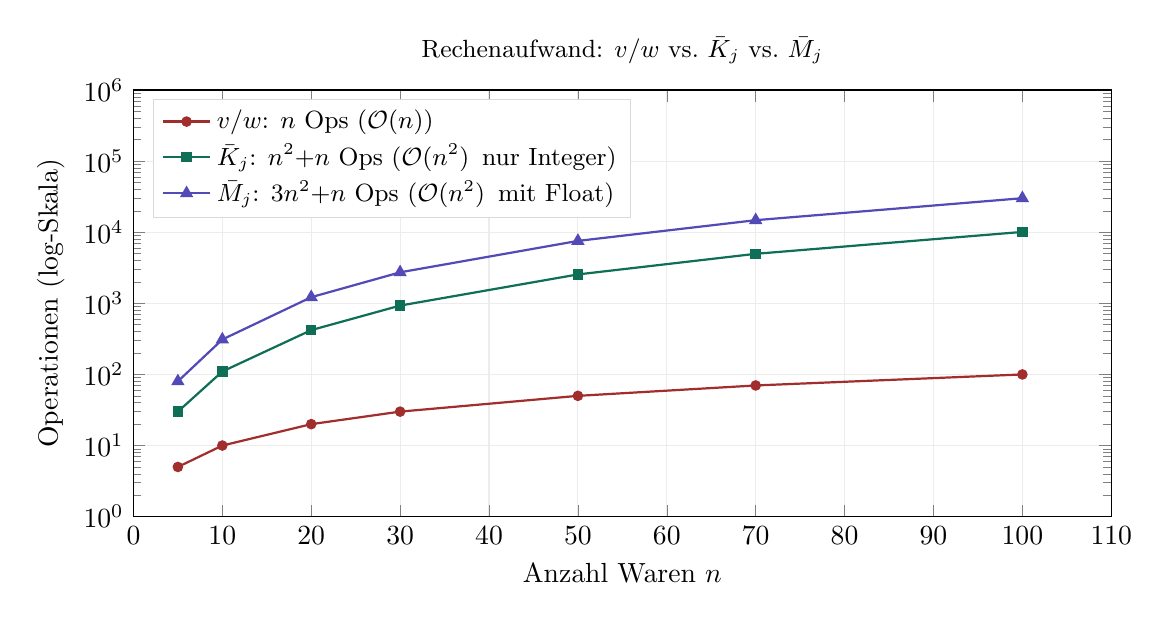
\begin{tikzpicture}
\begin{axis}[
  width=14cm, height=7cm,
  xlabel={Anzahl Waren $n$},
  ylabel={Operationen (log-Skala)},
  ymode=log,
  xmin=0, xmax=110,
  ymin=1, ymax=1e6,
  grid=major, grid style={gray!15},
  legend style={
    at={(0.02,0.98)},anchor=north west,
    font=\small, fill=white, draw=gray!30},
  legend cell align=left,
  title={Rechenaufwand: $v/w$ vs.\ $\bar{K}_j$ vs.\ $\bar{M}_j$},
  title style={font=\small},
]
% v/w: n operations (all float)
\addplot[thick,redcol,mark=*,mark size=1.5] coordinates {
  (5,5)(10,10)(20,20)(30,30)(50,50)(70,70)(100,100)};
% K-bar: n^2 integer + n float
\addplot[thick,tealcol,mark=square*,mark size=1.5] coordinates {
  (5,30)(10,110)(20,420)(30,930)(50,2550)(70,4970)(100,10100)};
% M-bar: 3n^2 + n
\addplot[thick,matblue,mark=triangle*,mark size=2] coordinates {
  (5,80)(10,310)(20,1220)(30,2730)(50,7550)(70,14770)(100,30100)};
\legend{
  $v/w$: $n$ Ops ($\mathcal{O}(n)$),
  $\bar{K}_j$: $n^2{+}n$ Ops ($\mathcal{O}(n^2)$\, nur Integer),
  $\bar{M}_j$: $3n^2{+}n$ Ops ($\mathcal{O}(n^2)$\, mit Float)}
\end{axis}
\end{tikzpicture}
\end{center}

\subsection{Kosten-Nutzen-Abwägung}

\begin{center}
\renewcommand{\arraystretch}{1.3}
\begin{tabular}{lcccc}
\toprule
Variante & Komplexität & Ops bei $n{=}100$
  & Operationstyp & Information \\
\midrule
Greedy $v/w$
  & $\mathcal{O}(n)$
  & $100$
  & Gleitkomma
  & eindimensional \\
$\bar{K}_j$ (rein)
  & $\mathcal{O}(n^2)$
  & $10\,100$
  & \textbf{nur Integer}
  & Packungsstruktur \\
$\bar{M}_j$ (Kern)
  & $\mathcal{O}(n^2)$
  & $30\,100$
  & Integer + Float
  & \textbf{Ersetzungswert} \\
\bottomrule
\end{tabular}
\end{center}

\noindent
\textbf{Analyse.}
Der Schritt von $\bar{K}_j$ zu $\bar{M}_j$ verdreifacht die
Operationszahl (von $n^2+n$ auf $3n^2+n$), weil pro Zelle zwei
zusätzliche Gleitkommaoperationen ($v_j/v_i$ und die Multiplikation
mit $K[i][j]$) anfallen. Dieser Mehraufwand liefert den
\emph{Ersetzungswert} -- die Information, ob der Platz einer
Ware mit einer anderen \emph{wertvoller} genutzt werden kann.

\medskip
\noindent
\textbf{Wann reicht $\bar{K}_j$?}
Die reine Kapazitätsmatrix $K$ liefert die Packungsstruktur:
wie oft passt Ware~$j$ in den Platz jeder anderen Ware.
Für Instanzen, in denen die Werte stark mit den Gewichten
korrelieren ($v_i \approx c \cdot w_i$ für eine Konstante $c$),
gilt $v_j/v_i \approx w_j/w_i$, und $\bar{K}_j$ enthält
implizit die Wertrelation. In diesem Fall genügt die reine
Integer-Berechnung.

\medskip
\noindent
\textbf{Wann lohnt sich $\bar{M}_j$?}
Bei unkorrelierten oder schwach korrelierten Instanzen
(typisch in der Praxis: $v$ und $w$ sind unabhängig verteilt)
liefert der Ersetzungsfaktor $v_j/v_i$ die entscheidende
Differenzierung. Hier investiert man den dreifachen
Rechenaufwand -- bekommt aber pro Ware nicht nur die
Aussage ``passt $k$-mal rein'' ($K$), sondern
``passt $k$-mal rein und bringt dabei das $r$-fache
des Werts'' ($M$).

\medskip
\noindent
\textbf{Alle drei Varianten bleiben $W$-unabhängig} --
keine von ihnen verwendet die Rucksackkapazität.
Dies unterscheidet sie fundamental von DP
($\mathcal{O}(nW)$), das bei großem $W$ drastisch
langsamer wird.

% ═══════════════════════════════════════════════════════════
\section{Diskussion}

\subsection{Einordnung in die Knapsack-Theorie}

Der Matrix-Score operiert an der Schnittstelle zweier
Problemklassen: er verwendet einen UKP-Operator
($\lfloor w_i/w_j \rfloor$, die ganzzahlige Packungshäufigkeit)
als Informationsquelle für ein 0/1-Problem.
Diese Brücke zwischen UKP und 0/1-KP ist konzeptionell neu
und erklärt die drei zentralen Eigenschaften der Methode:

\begin{enumerate}[leftmargin=*]
  \item \textbf{$W$-Unabhängigkeit.}
    Alle publizierten exakten und approximativen Methoden
    skalieren mit $W$ \citep{kellerer2004,balev2008}.
    Der UKP-Operator $\lfloor w_i/w_j \rfloor$ benötigt
    keine Kapazitätsangabe -- er ist rein item-relational.
    Diese Eigenschaft überträgt sich auf den Kern-Score $\bar{M}_j$.

  \item \textbf{Blockierungserkennung ohne Strafparameter.}
    In der UKP-Literatur wird $\lfloor w_i/w_j \rfloor$ als
    binäre Dominanzregel verwendet: eliminiere Item~$j$, wenn
    ein Item~$i$ existiert mit $\lfloor w_i/w_j \rfloor \cdot v_j
    \le v_i$ \citep{kellerer2004,andonov2000}.
    Der Matrix-Score transformiert diese binäre Ja/Nein-Entscheidung
    in einen \emph{kontinuierlichen} Score: statt Elimination
    wird der Grad der Dominanz quantifiziert und über alle
    Paarungen gemittelt.
    Schwere Waren mit wenigen Containern ($|\mathcal{C}_j|$ klein)
    erhalten naturgemäß weniger UKP-Evidenz -- ihr Score
    konvergiert zum Diagonalwert $M[j][j] = 1$
    (Satz~\ref{satz:dom}).

  \item \textbf{Relationale statt absolute Bewertung.}
    Greedy $v/w$ bewertet jede Ware isoliert: $v_j/w_j$ hängt
    von keiner anderen Ware ab. Der Matrix-Score bewertet jede
    Ware \emph{im Kontext aller anderen}: $\bar{M}_j$ ist ein
    gewichteter Mittelwert über $n^2$ paarweise Beziehungen.
    Dies erzeugt Struktur\-information, die in $v/w$ nicht
    enthalten ist -- insbesondere die Asymmetrie der
    Container-Inhalt-Relation (Satz~\ref{satz:asym}).
\end{enumerate}

\subsection{Greedy $v/w$ als Spezialfall}

Bemerkenswert ist, dass $v/w$ als Spezialfall eines
relationalen Scores interpretiert werden kann: der
Quotient $v_j/w_j$ misst die ``Selbsteffizienz'' einer
Ware -- den Wert pro Gewichtseinheit \emph{innerhalb}
der Ware. Der Matrix-Score generalisiert dies zu einer
``Fremdeffizienz'': dem Wert pro Gewichtseinheit
\emph{im Container einer anderen Ware}.
Dass beide Methoden in vielen Instanzen dieselbe Auswahl
treffen, zeigt: die Selbsteffizienz ist oft ein guter
Proxy für die Fremdeffizienz. Aber in Blockierungsfällen
(Gegenbeispiel, Abschnitt~\ref{sec:gegen}) divergieren
die beiden Perspektiven -- und der relationale Ansatz
liefert die bessere Auswahl.

\subsection{Limitationen}

\begin{itemize}[leftmargin=*,topsep=2pt]
  \item Der Kern-Score $\bar{M}_j$ ist parameterfrei, aber die
    optionale Blockierungsstrafe (Abschnitt~\ref{sec:strafe})
    erfordert die Wahl eines Koeffizienten $\alpha$, dessen
    optimaler Wert instanzabhängig ist.
  \item Für stark korrellierte Instanzen ($v_i \approx w_i + c$)
    sinkt die Performance aller Heuristiken, einschließlich des
    Matrix-Scores, da $v_j/v_i \approx w_j/w_i$ und die
    Ersetzungswerte nahe der Kapazitätszahlen liegen.
  \item Die $\mathcal{O}(n^2)$-Komplexität ist für sehr große $n$
    ($> 10^5$) ein Nachteil gegenüber $\mathcal{O}(n \log n)$-Methoden.
    Die reine Kapazitätsmatrix $\bar{K}_j$
    (nur Ganzzahloperationen) bietet hier eine schnellere
    Alternative (Abschnitt~\ref{sec:runtime}).
  \item In vielen Instanzklassen liefert $\bar{M}_j$ dieselbe
    Auswahl wie Greedy $v/w$ -- der relationale Mehrwert liegt
    dann in der Strukturinformation der vollen Matrix, nicht
    in der Auswahl selbst.
\end{itemize}

\subsection{Offene Fragen}

\begin{enumerate}[leftmargin=*,topsep=2pt]
  \item \textbf{Approximationsgarantie.}
    Kann eine formale worst-case-Güte für den Matrix-Score
    bewiesen werden? Für Greedy $v/w$ ist bekannt, dass die Güte
    beliebig schlecht werden kann \citep{kellerer2004}.
    Die empirischen Daten legen nahe, dass der Matrix-Score bei
    heterogenen Gewichten konsistent besser abschneidet.
  \item \textbf{Wertmatrix als zweite Dimension.}
    Die Kapazitätsmatrix $K_v[i][j] = \lfloor v_i/v_j \rfloor$
    liefert eine komplementäre Perspektive (``wie oft passt
    der Wert von $j$ in den Wert von $i$?''). Ob die Kombination
    von Gewichts- und Wertmatrix systematische Vorteile bietet,
    ist eine offene Forschungsfrage.
  \item \textbf{Mehrdimensionale Erweiterung.}
    Der UKP-Operator $\lfloor w_i/w_j \rfloor$ kann für
    jede Kapazitätsdimension (Gewicht, Volumen, Energie, \ldots)
    separat berechnet werden. Die Kombination mehrerer
    Proportionsmatrizen zu einem Multi-Constraint-Score
    ist ein natürlicher Erweiterungspfad.
\end{enumerate}

% ═══════════════════════════════════════════════════════════
\section{Fazit}

Diese Arbeit stellt eine neue Perspektive auf das 0/1-Knapsack-Problem
vor: die Bewertung von Waren nicht durch isolierte Effizienzquotienten,
sondern durch ihre \emph{relationale Stellung im Warenkollektiv}.

\begin{mdframed}[backgroundcolor=matlight,linecolor=matblue,linewidth=1.2pt]
\textbf{Der Kern-Score $\bar{M}_j$} -- der mittlere Ersetzungswert
über alle aufnehmenden Container -- ist:
\begin{itemize}[leftmargin=*,topsep=4pt]
  \item \textbf{parameterfrei}: keine empirischen Koeffizienten,
    keine Kalibrierung, vollständig reproduzierbar,
  \item \textbf{$W$-unabhängig}: das einzige nicht-triviale
    Bewertungsverfahren in der Knapsack-Literatur, das die
    Kapazität $W$ in keiner Berechnung verwendet,
  \item \textbf{UKP-informiert}: nutzt den Dominanzoperator
    $\lfloor w_i/w_j \rfloor$ aus der Unbounded-Knapsack-Theorie
    \citep{kellerer2004,andonov2000} nicht zur Eliminierung,
    sondern als Baustein einer relationalen Bewertung --
    eine Brücke zwischen UKP und 0/1-KP, die in der Literatur
    nicht vorhanden ist,
  \item \textbf{strukturell aufschlussreich}: die volle
    $n \times n$-Matrix liefert paarweise Ersetzungswerte,
    Blockierungsinformation, Dominanzverhältnisse und
    Container-Inhalt-Asymmetrien -- Information, die über die
    bloße Warenauswahl hinausgeht.
\end{itemize}
\end{mdframed}

\medskip
\noindent
\textbf{Was der Matrix-Score leistet.}
Im konstruierten Gegenbeispiel (Abschnitt~\ref{sec:gegen})
findet der reine Kern-Score $\bar{M}_j$ das DP-Optimum (134\,\euro),
wo die $v/w$-Heuristik durch einen Blockierer scheitert (130\,\euro).
Dies gelingt ohne Strafparameter -- allein durch die relationale
Struktur der Proportionsmatrix: die schwerste Ware erhält
naturgemäß wenige Container ($|\mathcal{C}_j| = 1$) und damit
wenig UKP-Evidenz.

\medskip
\noindent
\textbf{Was der Matrix-Score nicht leistet.}
In vielen Instanzklassen liefert $\bar{M}_j$ dieselbe Auswahl
wie der einfachere Greedy $v/w$ -- der Mehraufwand $\mathcal{O}(n^2)$
gegenüber $\mathcal{O}(n \log n)$ wird dann nicht durch eine
bessere Auswahl gerechtfertigt. Der Wert der Methode liegt in
diesen Fällen nicht im Ergebnis, sondern in der
\emph{Transparenz}: die Proportionsmatrix macht sichtbar,
\emph{warum} eine Ware gut oder schlecht ist -- nicht nur
\emph{dass} sie es ist.

\medskip
\noindent
\textbf{Ausblick.}
Die relationale Matrixmethode eröffnet drei Forschungsrichtungen:
(1)~die formale Charakterisierung der Instanzklassen, in denen
$\bar{M}_j$ von $v/w$ abweicht,
(2)~die Erweiterung auf mehrdimensionale Knapsack-Probleme durch
separate Proportionsmatrizen pro Kapazitätsdimension,
(3)~die Nutzung der Wertmatrix $K_v[i][j] = \lfloor v_i/v_j \rfloor$
als komplementäre Informationsquelle.
Der Grundgedanke -- jede Ware gleichzeitig als Container
\emph{und} als Inhalt zu betrachten -- ist auf verwandte
kombinatorische Optimierungsprobleme (Bin Packing,
Scheduling, Portfolio-Selektion) übertragbar.

% ═══════════════════════════════════════════════════════════
\bibliographystyle{plainnat}
\bibliography{knapsack}

% ═══════════════════════════════════════════════════════════
\clearpage
\begin{appendices}
\section{Schritt-für-Schritt-Anleitung}
\label{app:anleitung}

Diese Anleitung zeigt, wie der Matrix-Score für eine beliebige
Knapsack-Instanz berechnet wird.

\subsection*{Voraussetzungen}

Gegeben: $n$ Waren mit Werten $v_1,\ldots,v_n > 0$
und Gewichten $w_1,\ldots,w_n > 0$, sowie Kapazität $W > 0$.

\subsection*{Schritt 1: Eingabetabelle erstellen}

Trage alle Waren in eine Tabelle ein.
Berechne für jede Ware das Verhältnis $v_i/w_i$.

\begin{center}
\small
\begin{tabular}{ccccc}
\toprule
$j$ & Bezeichnung & $v_j$ & $w_j$ & $v_j/w_j$ \\
\midrule
1 & \ldots & \ldots & \ldots & \ldots \\
\vdots & & & & \\
$n$ & \ldots & \ldots & \ldots & \ldots \\
\bottomrule
\end{tabular}
\end{center}

\subsection*{Schritt 2: Kapazitätsmatrix $K$ aufstellen}

Erstelle eine $n \times n$-Tabelle. Berechne für jede Zelle:
\[
K[i][j] = \left\lfloor \frac{w_i}{w_j} \right\rfloor
\]
\textit{Tipp:} Beginne mit der Diagonale ($K[i][i] = 1$ für alle $i$).
Alle Zellen mit $w_j > w_i$ sind automatisch~$0$.

\subsection*{Schritt 3: Proportionsmatrix $M$ berechnen}

Multipliziere jede Zelle mit dem Wertverhältnis:
\[
M[i][j] = K[i][j] \cdot \frac{v_j}{v_i}
\]
\textit{Tipp:} Die Diagonale bleibt $M[i][i] = 1{,}00$.
Alle Nullen aus $K$ bleiben Nullen in $M$.

\subsection*{Schritt 4: Score pro Ware berechnen}

Für jede \emph{Spalte} $j$:
\begin{enumerate}[topsep=2pt]
  \item Zähle die Nicht-Null-Einträge in Spalte $j$
    (alle $i$ mit $\lfloor w_i/w_j \rfloor > 0$):
    das ist $|\mathcal{C}_j|$.
  \item Berechne den Mittelwert der Nicht-Null-Einträge:
    \[
    \operatorname{Score}(j) = \bar{M}_j = \frac{1}{|\mathcal{C}_j|}
    \sum_{i \in \mathcal{C}_j} M[i][j]
    \]
\end{enumerate}

\noindent
\textit{Optional:} Für Instanzen mit dominanten schweren Items
kann die Blockierungsstrafe aktiviert werden
(vgl.\ Abschnitt~\ref{sec:strafe}):
$\operatorname{Score}_\alpha(j) = \bar{M}_j \cdot
(1 - \alpha \cdot |\mathcal{Z}_j|/n)$
mit $\mathcal{Z}_j = \{i : \lfloor w_i/w_j \rfloor = 0\}$.

\subsection*{Schritt 5: Waren auswählen}

\begin{enumerate}[topsep=2pt]
  \item Sortiere die Waren absteigend nach Score.
  \item Gehe die sortierte Liste durch:
    \begin{itemize}[topsep=2pt]
      \item Falls die Ware noch in den Rucksack passt
        ($w_j \le W_{\text{rest}}$): aufnehmen,
        $W_{\text{rest}}$ reduzieren.
      \item Sonst: überspringen.
    \end{itemize}
  \item Ergebnis: die Menge $S$ der ausgewählten Waren.
\end{enumerate}

\subsection*{Checkliste}

\begin{center}
\small
\begin{tabular}{lcc}
\toprule
Prüfpunkt & Erwartet & $\checkmark$ \\
\midrule
Diagonale von $M$ & alle $= 1{,}00$ & \\
$M[i][j] = 0$ wenn $w_j > w_i$ & alle Nullen korrekt & \\
$|\mathcal{C}_j| \ge 1$ für jedes $j$ & ja (mind.\ Diagonale) & \\
$\bar{M}_j > 0$ für alle Waren & ja & \\
Gesamtgewicht der Auswahl $\le W$ & ja & \\
\bottomrule
\end{tabular}
\end{center}

\end{appendices}

\end{document}
